\chapter{Implementation}\label{chap:impl}
In this chapter, my goal is to reveal the details of the implementation for all the experiments described in the methodology~\ref{chap:met}. My description will include the algorithm to convert the text data into a format for efficient training with the transformer model. It also includes details about the hyperparameters that I used for the training and the generation process. This chapter will also cover the architecture-specific details for the experiments with custom modules. Each section of this chapter concludes with the results of the experiment and a summary of the training process.
\section{Vanilla CodeT5+ training details}
The theoretical aspects of training the transformer-based encoder-decoder model for the commit message generation task were described in the corresponding methodology section \ref{sec:codeT5_train}, and in this part of the work, I will give details of the implementation of the training process. This section includes details of the model input sequence format and the representation of the label vector to compute the loss function. In addition, I will describe the hyperparameters required for model training and inference and the logic behind them.
\subsection{Input sequences representation}
The first step in training a neural network involves preparing and converting the data into the input format of the model. CommitChronicle dataset stores code changes in the format of JSON. It is required to convert it into plain text and insert special tokens in the data preprocessing stage, according to the desired format \ref{sec:structure_of_the_data}. 
The next step in data preparation is to tokenize the text. Machine learning models cannot process data in text format because they can only work with numeric values.
Initially, I needed to convert text into numbers. The standard method is to use a pre-trained tokenizer that is trained with the model. The tokenizer contains a vocabulary with the mapping of words to numbers. The model takes a sequence of numbers as input, each corresponding to a word in the dictionary.
In neural network training, data are typically passed in batches rather than as a single sequence. Batched training is utilized to accelerate GPU computations and improve loss convergence. For this reason, the input batch should have the form of a matrix. The issue of constructing this matrix arises due to the varying lengths of the input sequences. This condition makes it impossible to unify the shape of the batch matrix without additional data transformation. The common technique to resolve this issue in the sequence processing task is to add padding tokens to each sample to equalize all sequences in length. These padding tokens are excluded from the model's self-attention calculation, so expanding the sequence length does not result in additional computations. For my experience with CodeT5+, I expanded all the input sequences to the maximum size of the model context, 512 tokens. The same padding should be applied to the label vectors. The difference is that the cross-entropy loss interprets the padding as correctly guessed tokens, thus making the loss function less sensitive. To avoid this loss degradation, I excluded padding tokens while computing it.
All the techniques described in this section are required for the efficient interpretation of the data by the model. Furthermore, this preprocessing enables the batched model training and the efficient loss computation.

\subsection{Training hyper-parameters}
The choice of hyper-parameters is the crucial step in neural network training. The performance of a model in a given task is significantly impacted by a set of hyperparameters that affect the convergence of the loss function. In this section, I will describe all the hyperparameters chosen to fine-tune the CodeT5+ model for the commit message generation task. In addition, I will define each parameter and explain how they affect the fine-tuning process.
\setcounter{table}{4}
\begin{table}[h]
    \centering
    \caption{Fine-tuning hyper-parameters choice}\label{tab:ft_hyperparams}
    \renewcommand{\arraystretch}{1.5} % Adjusts the row height
    \begin{tabular}{| l | c |} % chktex 44
    \hline % chktex 44
    \textbf{Hyper-parameter} & \textbf{value} \\
    \hline % chktex 44
    batch size      & $32$ \\ \hline  
    optimizer       & AdamW \\ \hline  
    learning rate     & $2 \times 10^{-5}$ \\ \hline  
    learning rate scheduler & linear \\ \hline
    weight decay       & $10^{-2}$ \\ \hline  
    warm-up steps & $100$ \\ \hline  
    warm-up strategy & linear \\ \hline
    bf16    & True \\ \hline  
    \end{tabular}
\end{table}
Table~\ref{tab:ft_hyperparams} represents a list of all hyper-parameter configurations for CodeT5+ fine-tuning. The \textbf{batch size} for training and evaluation was set to 32. According to empirical findings, this batch size is optimal in training time and computing resource usage. As an \textbf{optimizer} I chose an improved version of Adam Optimizer~\cite{kingma2014adam} that decouples weight decay from the optimization steps, applying it directly to the weights - AdamW~\cite{loshchilov2017decoupled}. In recent research, it has been shown that this optimizer leads to better convergence in the task of causal language modeling. For the \textbf{learning rate} I set the maximum value at $2 \times 10^{-5}$. The learning rate can be interpreted as a "step size" for the gradient descent method. In general form, it corresponds to $\gamma$ in the update formula of the model parameters $w_{\text{new}} = w_{\text{old}} - \gamma \nabla f(w_{\text{old}})$. During training, the learning rate is configured using the \textbf{linear scheduler}, which monotonically decreases the learning rate to 0 until the end of training. One more parameter to configure the learning rate is the \textbf{linear warm-up}, which monotonically increases it to the maximum specified by the current from 0 during the \textbf{warm-up steps}. \text{Weight decay} is the hyperparameter responsible for the regularization of the parameters of the neural network. The optimization objective then takes the form of $L_{\text{new}(w)} = L_{\text{original}}(w) + \lambda w^Tw$, where $\lambda$ is the specified strength of the weight decay penalty. The hyperparameter \textbf{ bf16} indicates that instead of full precision with 32-bit float model parameters and optimizer states, I used brain float with 16 bits. Bfloat differs from the usual half-precision float in that it has 8 bits in the exponent part, while fp16 has only 5 bits. With this modification, bfloat16 can handle the same range of numbers as a full-precision float with 32 bits but with less precision than fp16, as it has fewer bits in mantissa. Recent research~\cite{kalamkar2019study} has shown that the training of neural networks with bf16 achieves the same performance as the full precision but with fewer computational resources required. 
All the hyper-parameters described above are used to configure the training process. The set of parameters in this section, except for batch size, is shared among all models trained in my work. This set of parameters was taken from~\cite{eliseeva2023commit}, as the authors of this work achieved SOTA on the commit message generation task using the same dataset.

\subsection{Generation hyper-parameters}
The output of a trained language model represents the probability distribution of the next text token. To construct an output, the model predicts all tokens in an autoregressive manner. This means that when predicting the output $\hat{Y}$, $\hat{y}_n$ depends on the previously generated context $(\hat{y}_0 \dots \hat{y}_{n-1})$. One of the possible ways to construct an output sequence is to choose the most probable token every time. However, this greedy strategy may lead to the degradation of the generated text. There exist methods to make the generated text more human-readable and increase the cumulative probabilities of the choices. In this section, I will describe the generation hyperparameters that I used for my model and explain the intuition behind them to justify my choice.

\begin{table}[h]
    \centering
    \caption{Generation hyper-parameters choice}\label{tab:gen_hyperparams}
    \renewcommand{\arraystretch}{1.5} % Adjusts the row height
    \begin{tabular}{| l | c |} % chktex 44
    \hline % chktex 44
    \textbf{Hyper-parameter} & \textbf{value} \\
    \hline % chktex 44
    max new tokens & $128$ \\ \hline
    top k & $100$ \\ \hline
    number of beams & $5$ \\ \hline
    early stopping & True \\ \hline
    no-repeat n-gram size & $2$ \\ \hline
    do sample & True \\ \hline
    top p & $0.95$ \\ \hline 
    \end{tabular}
\end{table}

Table~\ref{tab:gen_hyperparams} lists the set of hyperparameters that I use to generate commit messages. \textbf{Max new tokens} configures the maximum length of the generated message. According to the statistics of the training dataset, the commit messages are $\sim60$ characters on average. To make the results similar to the actual message, I limited the maximum number of generated tokens. \textbf{Top k} parameter is responsible for the number of tokens that the model considers in the prediction. It makes the model choose only among the k most probable words. This technique prevents the model from hallucinating by randomly selecting the inappropriate token, making the generation more stable. The parameter \textbf{ number of beams} refers to the beam search decoding strategy. It implies the use of heuristics to make the output more diverse. Each beam starts from the initial position and predicts the next token according to the probabilities of the model. At the end of the generation, the beams are reranked according to the cumulative probability of the predicted sequences. \textbf{Early stopping} flag also corresponds to beam search. It controls that the generation process should stop after the first \textbf{num\_beams} beams are done. 
I also prevented the model from generation of the same bigram several times. It is a known issue of large language models that they may hallucinate and start repeating some phrase until the end of the response. 
\textbf{Do sample} parameter just states what tokens are selected according to the probabilities, and not just with a greedy strategy.
\textbf{Top p} parameter corresponds to the nucleus sampling method proposed in~\cite{holtzman2019curious}. According to this method, only the smallest set of most probable tokens with probabilities that add up to \textbf{top\_p} or higher are kept for generation. This technique is similar to \textbf{top\_k} and prevents the model from hallucinating and predicting irrelevant tokens.
All of the generation hyperparameters described in this section help the model generate more relevant text. Moreover, some of the parameters, like sampling, make the generated commit message more human-readable. 

\subsection{Training process}
In this section, I will describe the details of the training process for the base version of CodeT5+~\cite{wang2023codet5+} with 220 million parameters. As training data, I took the train split from the CommitChronicle data set~\cite{eliseeva2023commit} and for the intermediate evaluation, I took the subset of the CommitChronicle validation set with 1500 random samples. I trained my model for one epoch with the use of 2 NVIDIA A100 80GB. In total, the training process took 3 days and 19 hours. 

\begin{figure}[H]
    % \hspace*{-1.5cm}
    \centering
    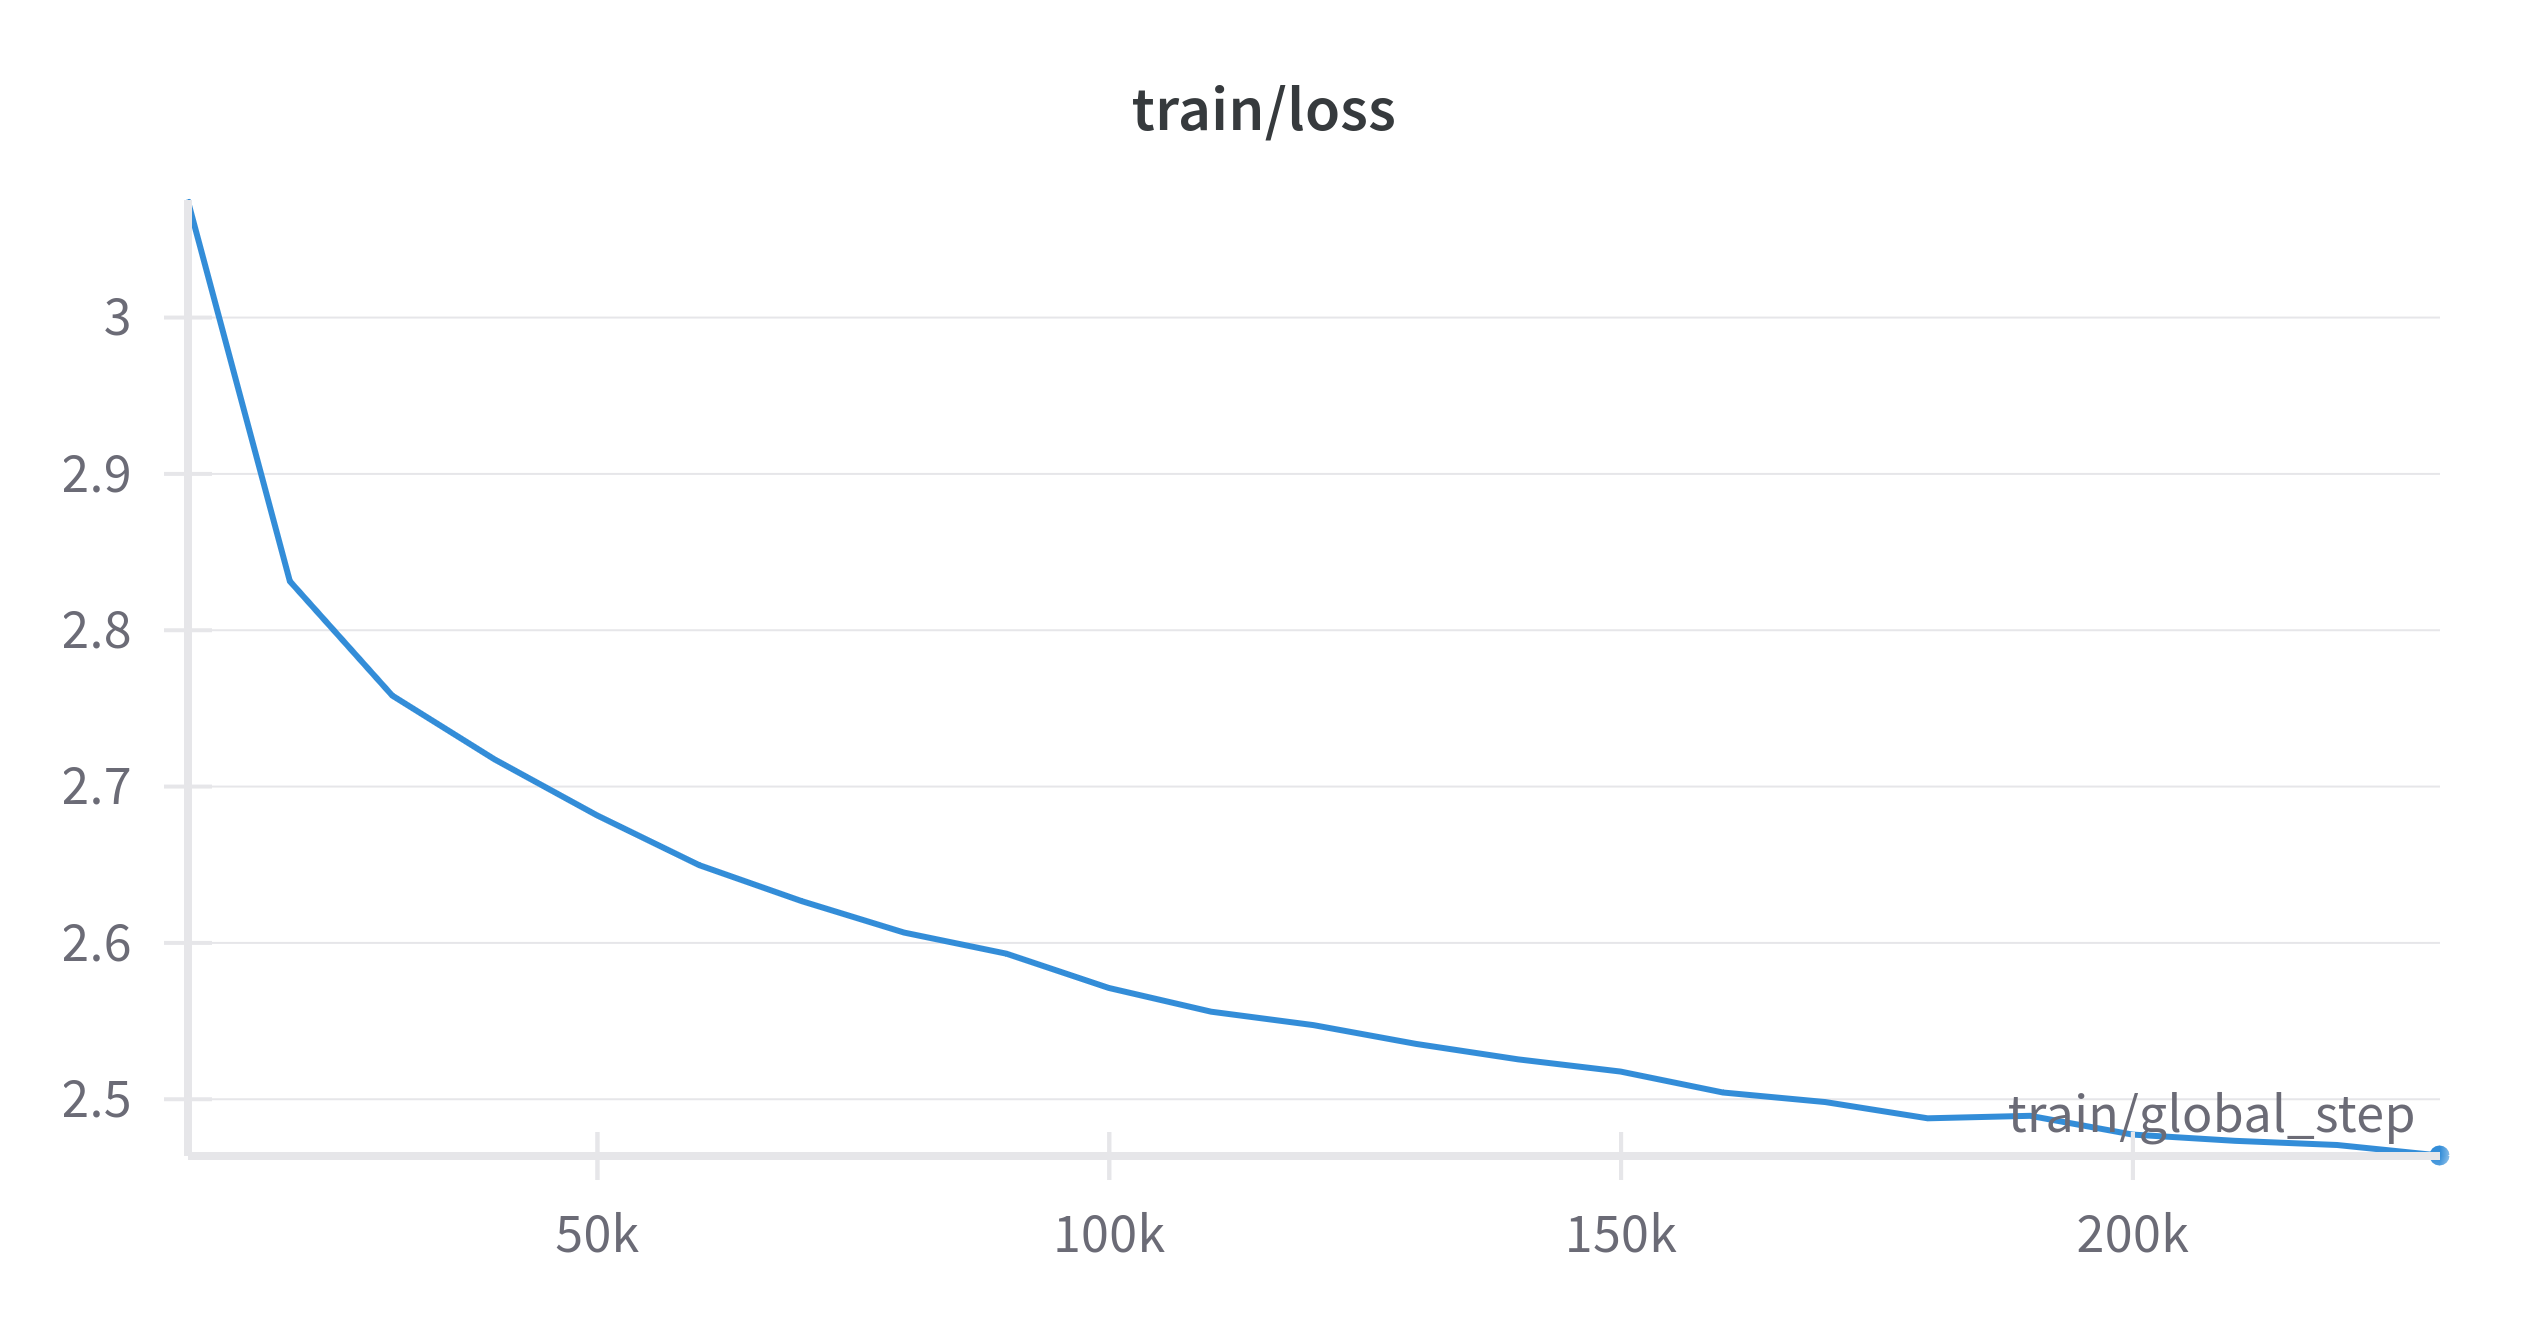
\includegraphics[scale=0.15]{figs/train_loss_base.png} \\
    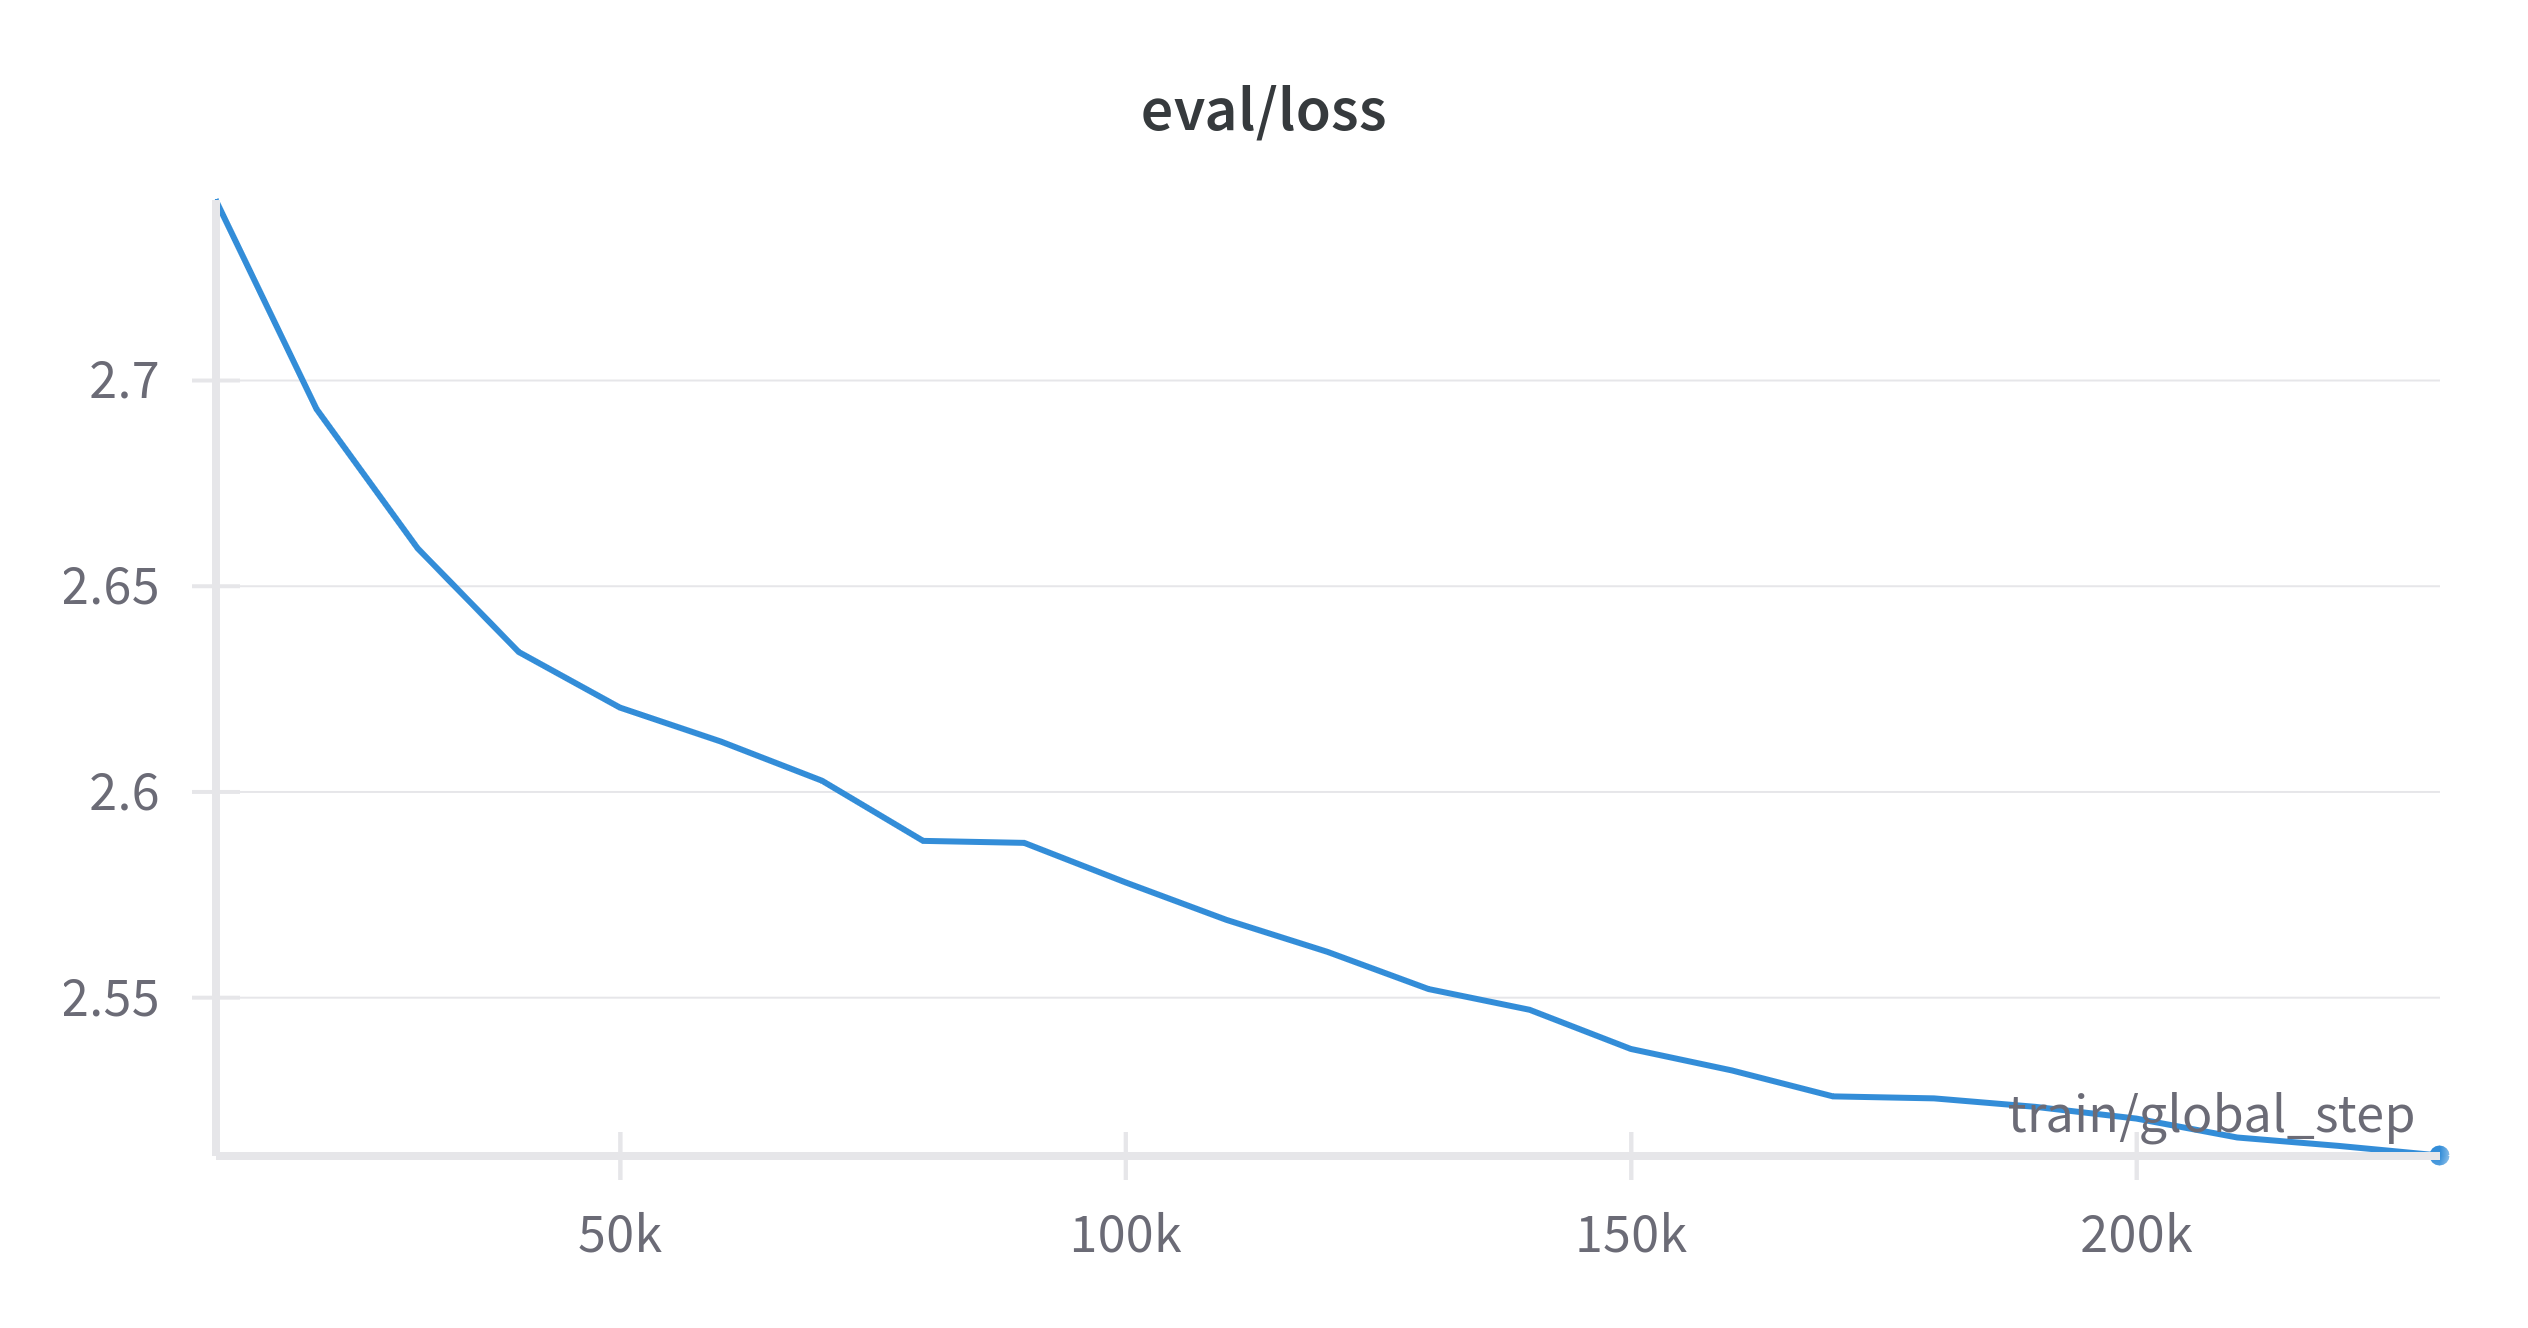
\includegraphics[scale=0.15]{figs/val_loss_base.png}
    \caption{Loss history for the base model.}
    ~\label{fig:base_model_loss}
\end{figure}
Results of the loss behaviour during the fine-tuning process are presented in~\ref{fig:base_model_loss}. From the plots, it is easy to see that the loss decreased during fine-tuning in both the training and validation sets. This means that the fine-tuning process was successful. The model improved its ability to generate commit messages for the training set and generalized this skill on the validation set.

\begin{figure}[H]
    \centering % Centers all content within the figure environment
    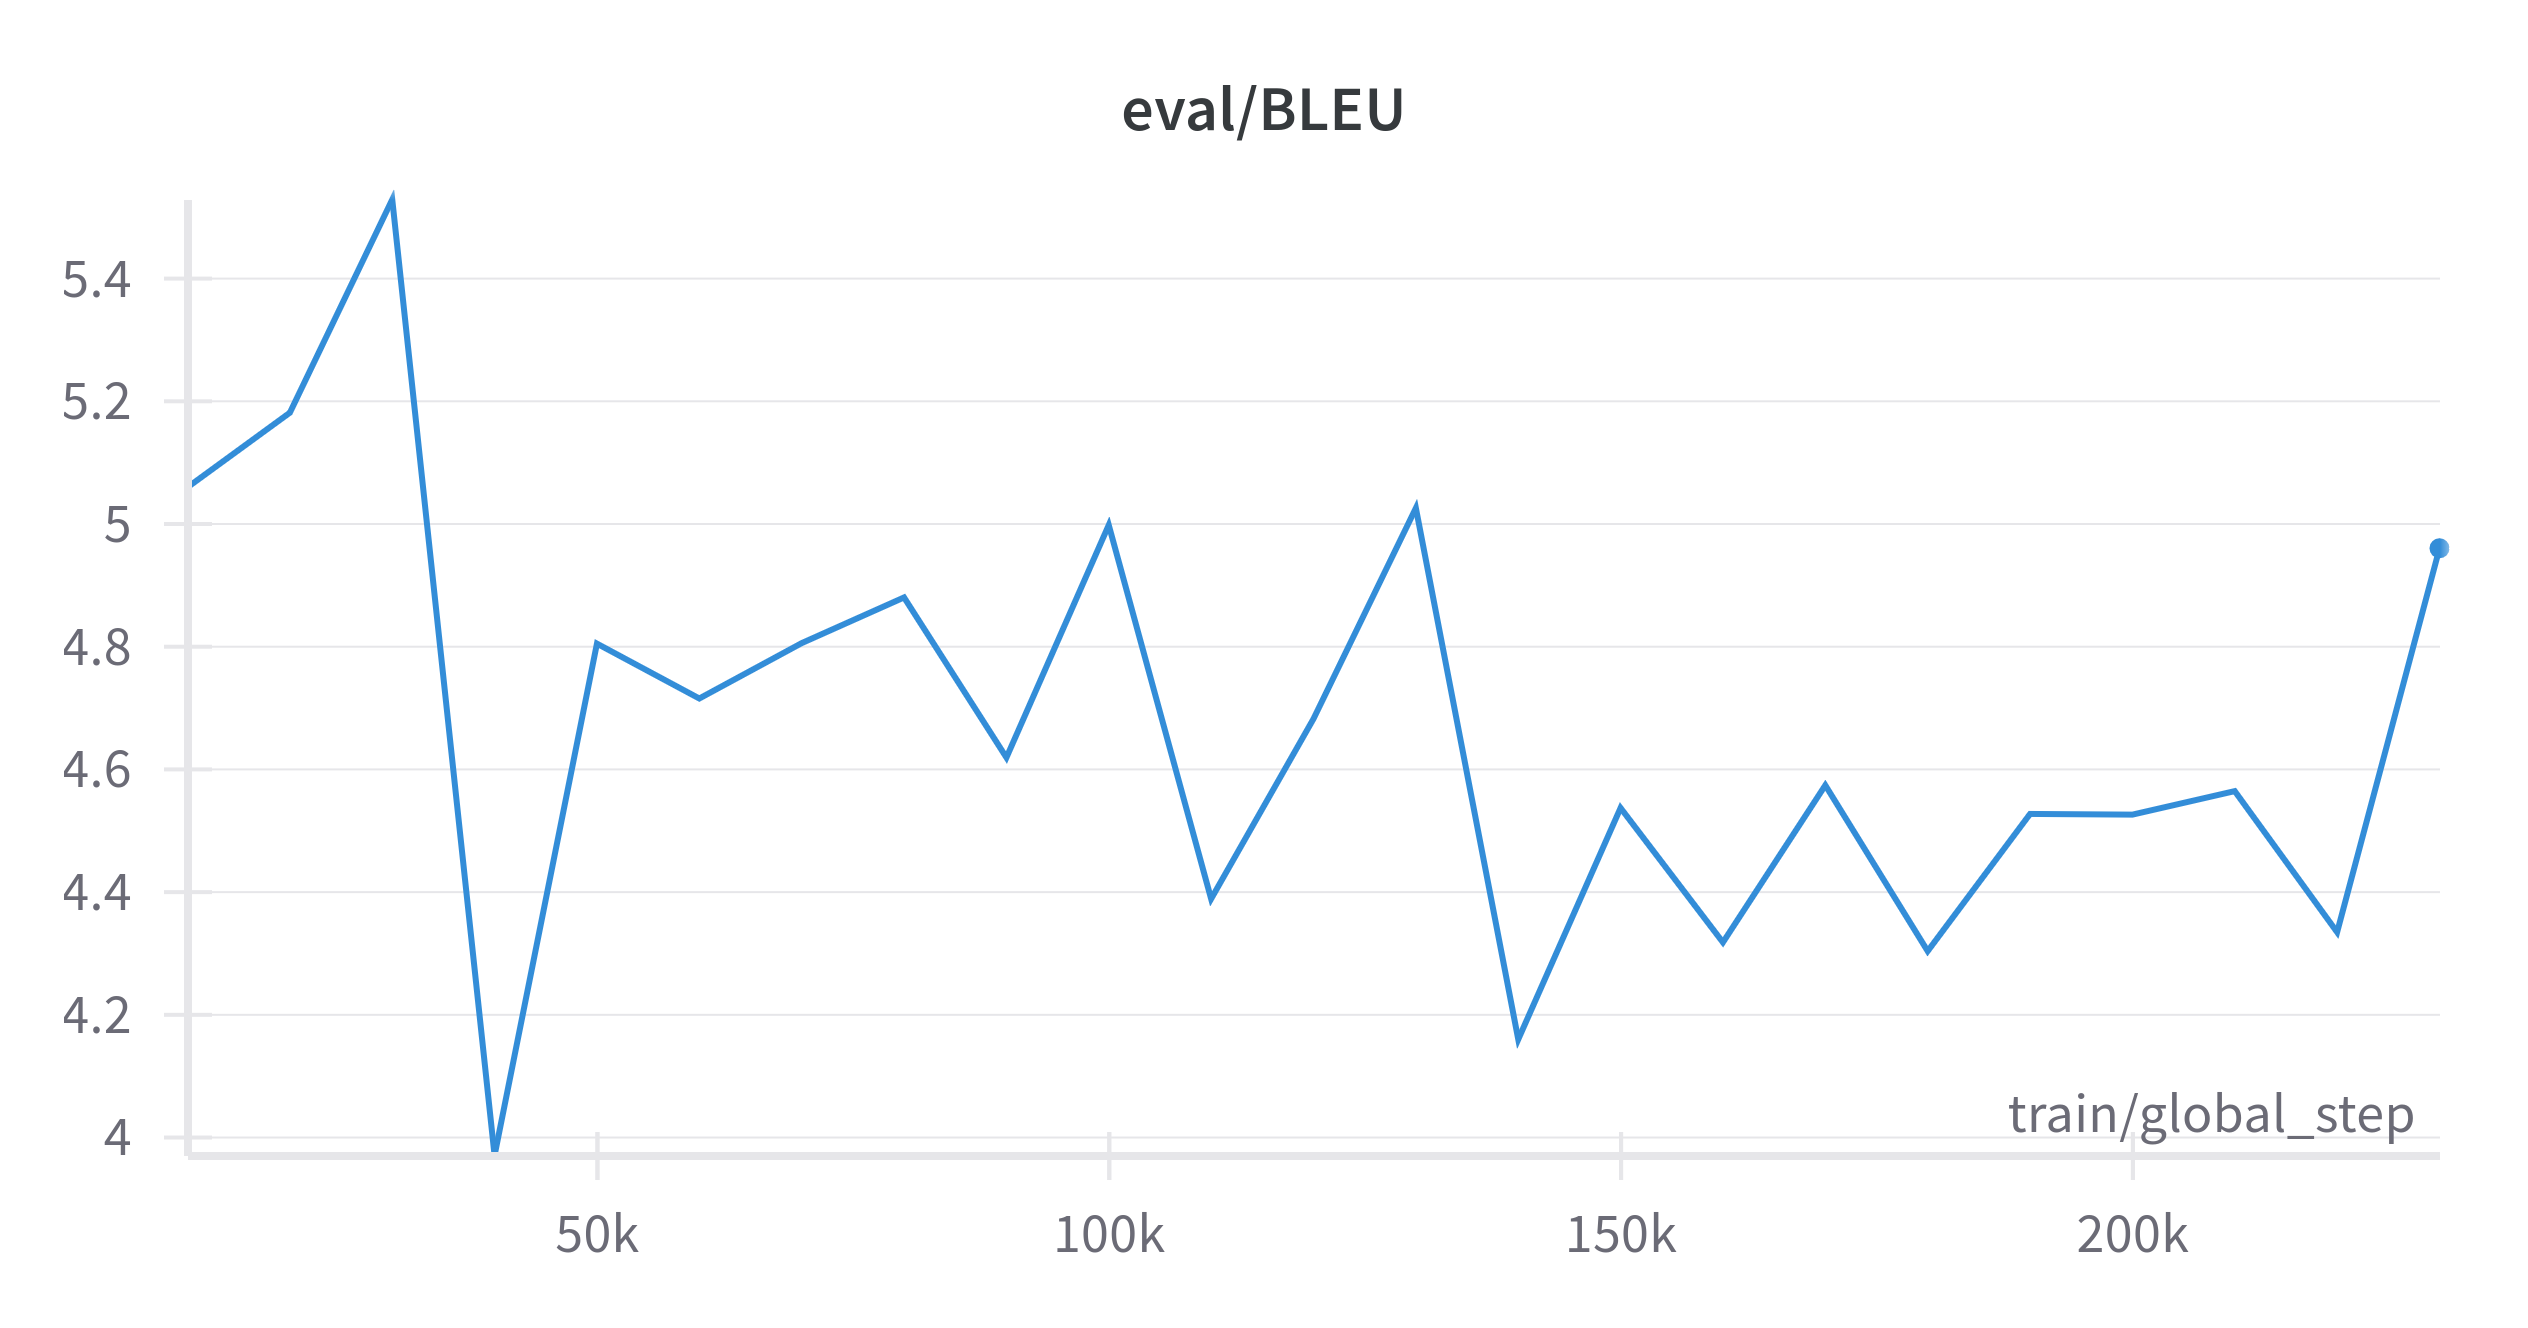
\includegraphics[scale=0.12]{figs/base_bleu.png} \\
    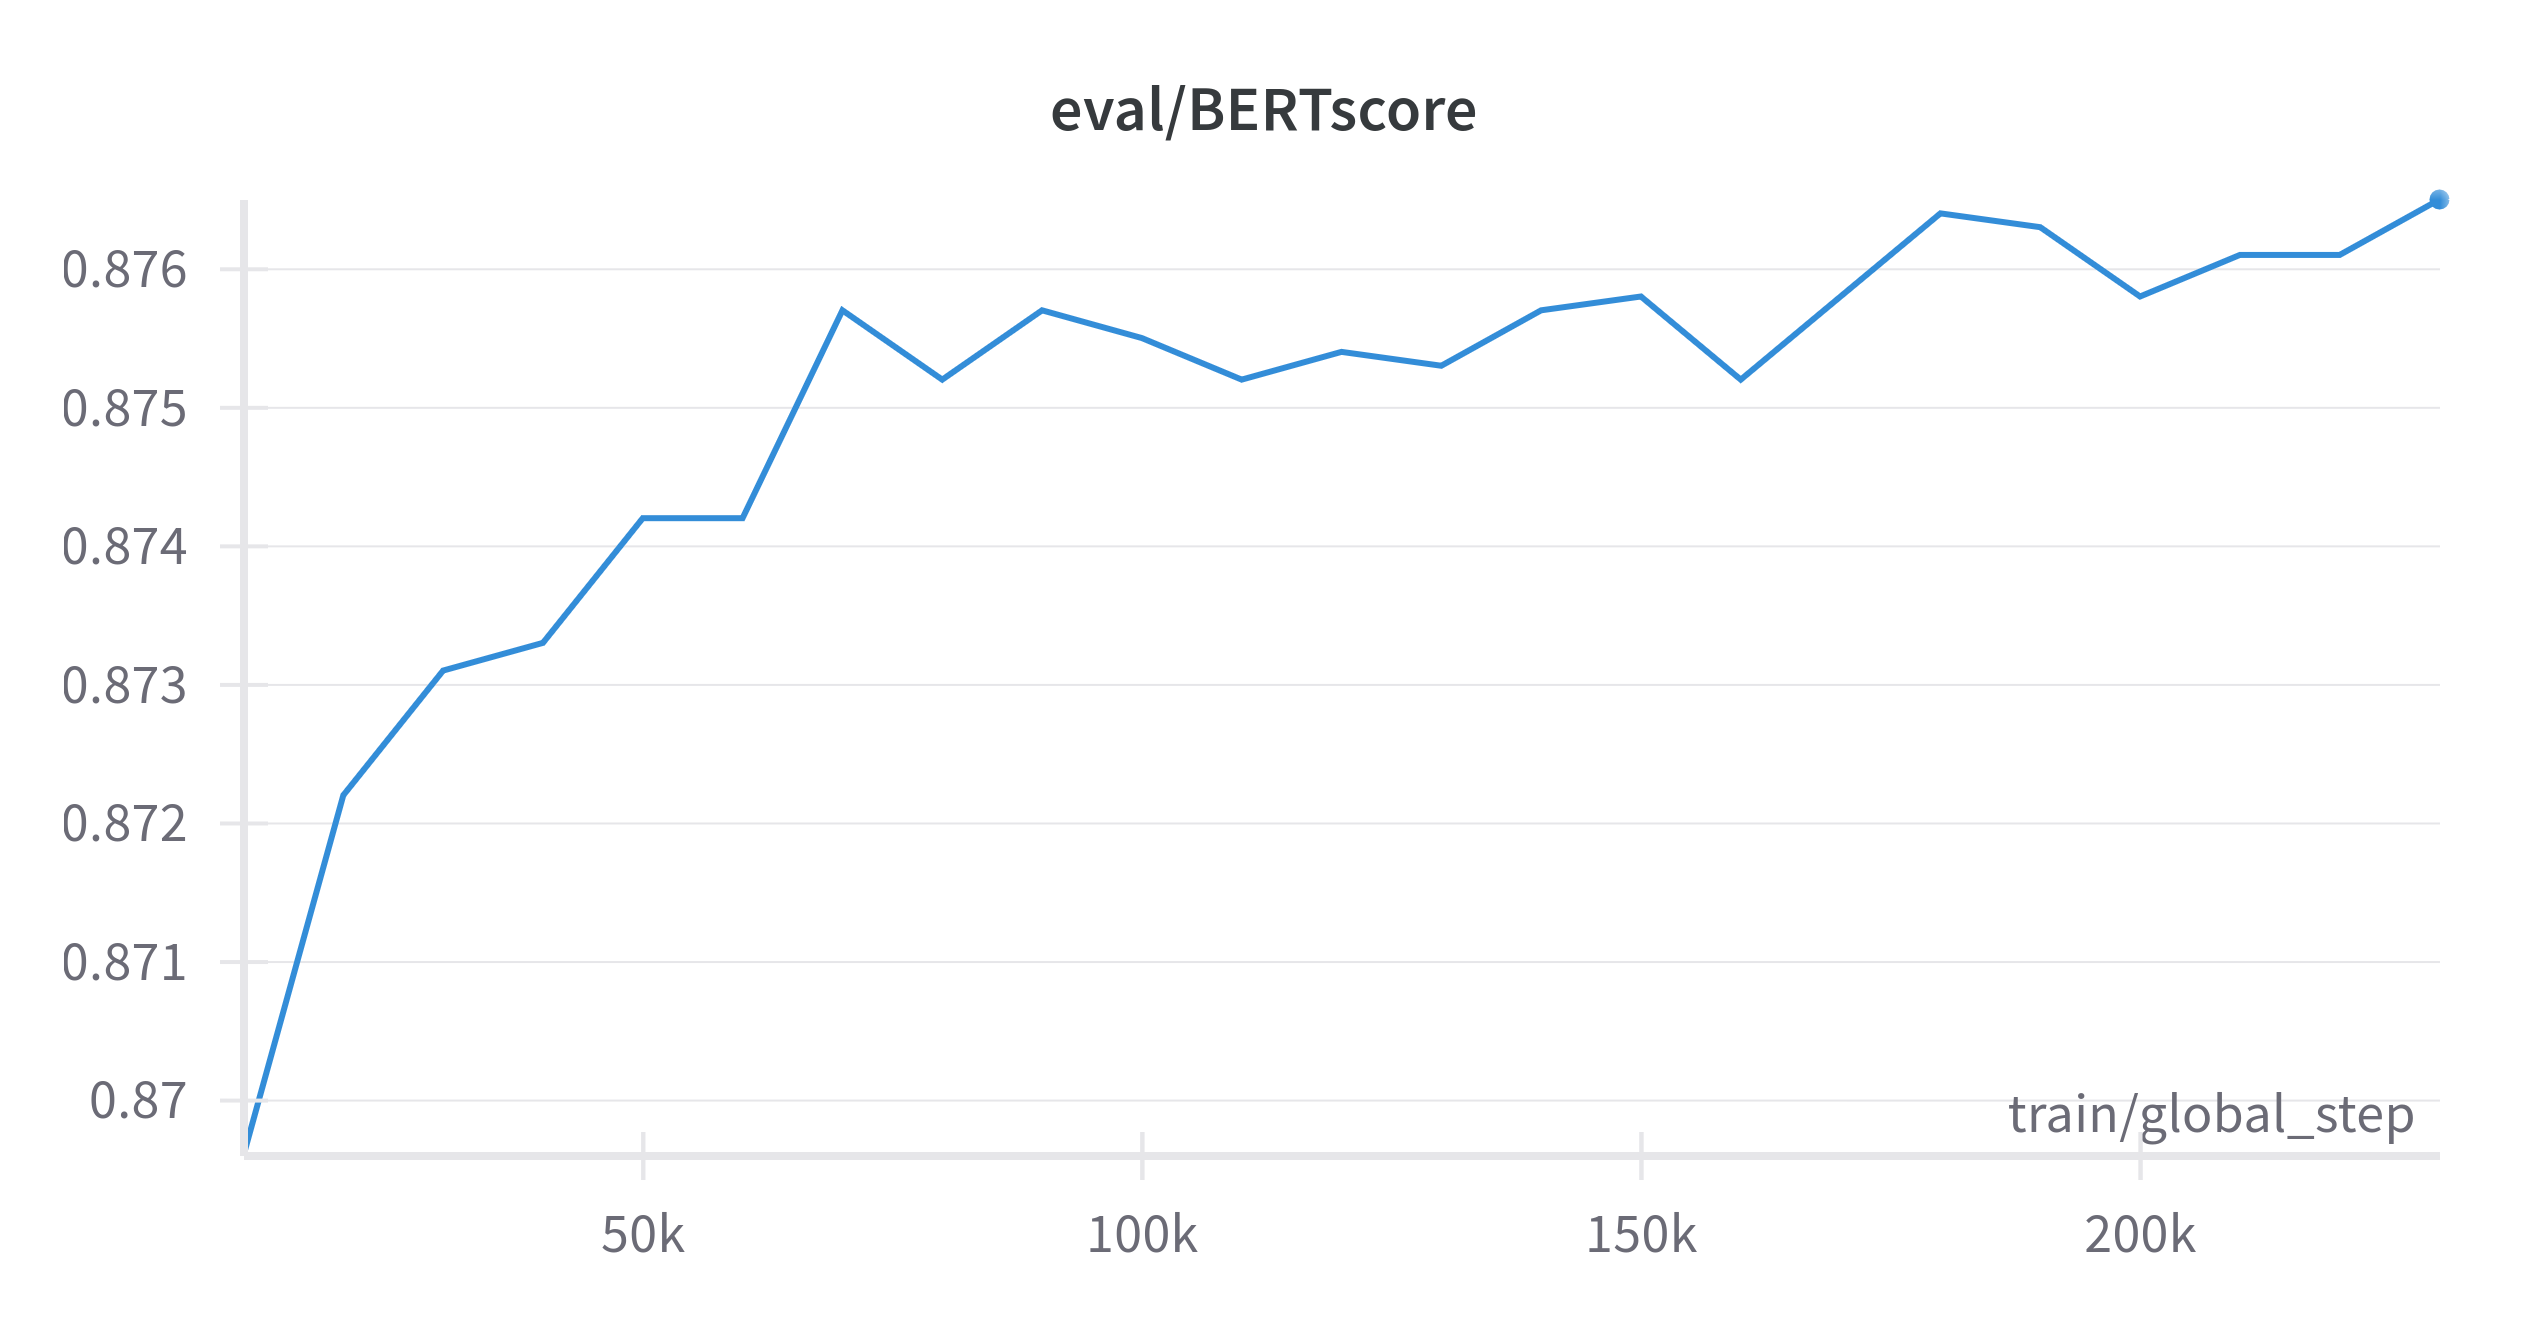
\includegraphics[scale=0.12]{figs/base_bertscore.png} \\
    % Adds a line break and centers the following image
    \centering 
    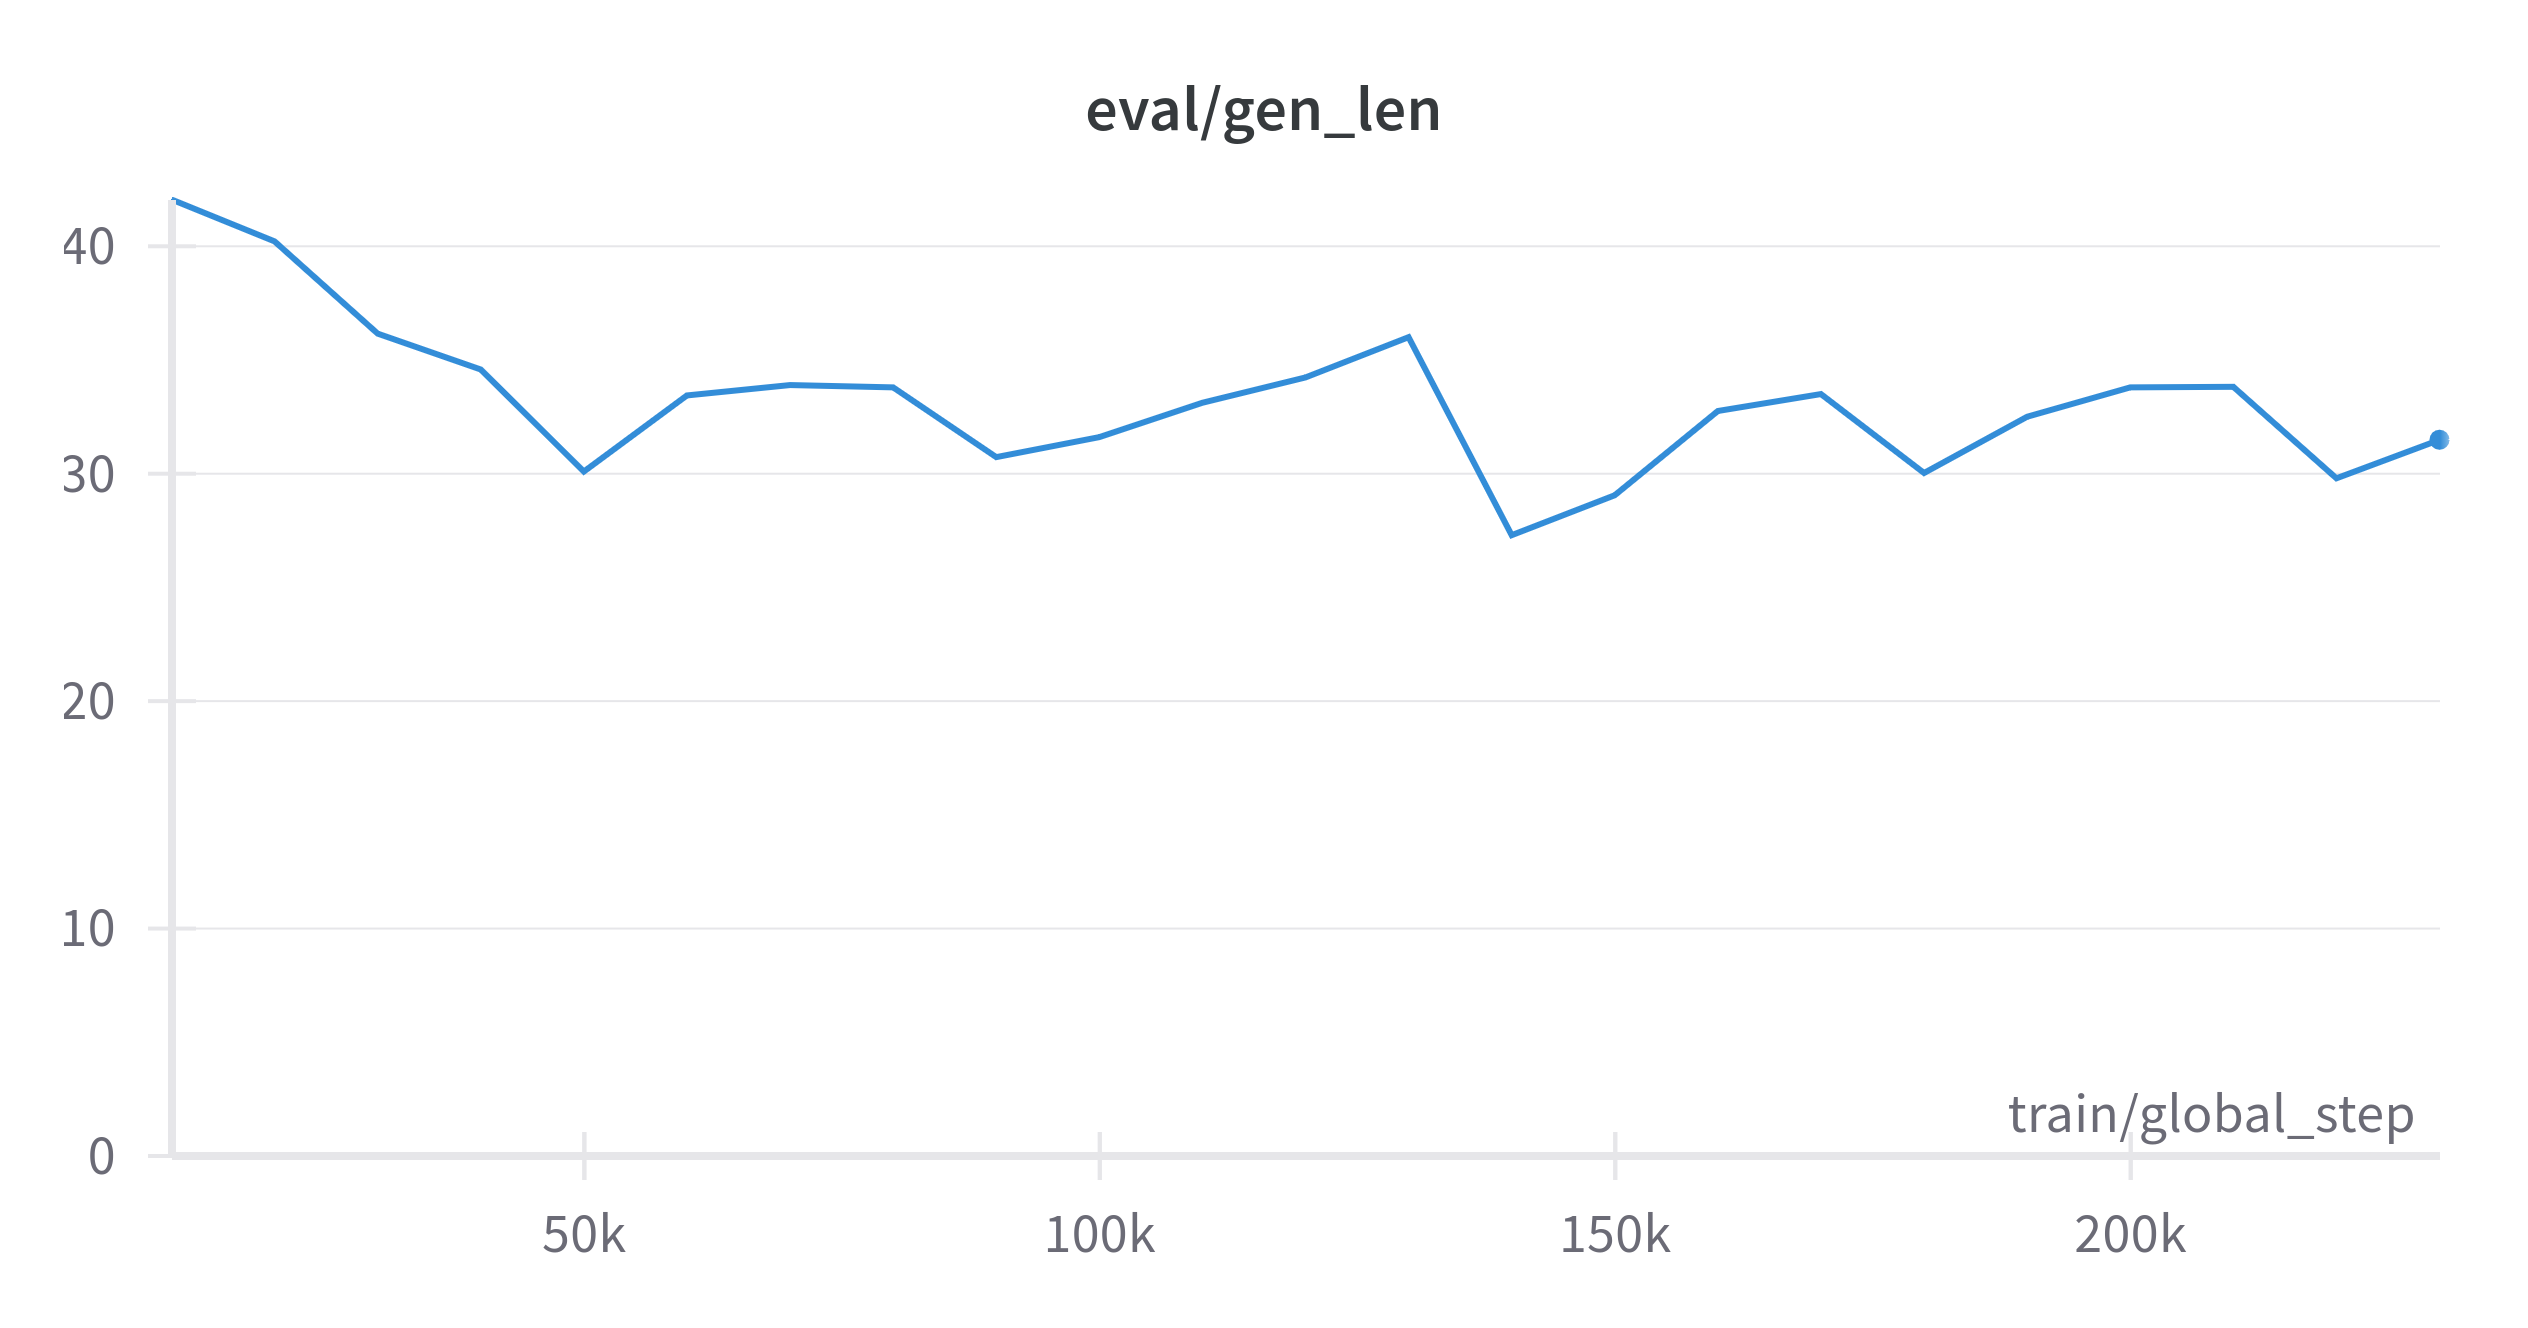
\includegraphics[scale=0.12]{figs/base_genlen.png}
    \caption{Evaluation results for the base model}
    \label{fig:base_model_interim_metrics}
\end{figure}

The results of the training are presented in Fig.~\ref{fig:base_model_interim_metrics}.  From the plots, it is visible that the BERTScore improved during the fine-tuning. This improvement signalled that the quality of the generated commit messages improved. But the range of the BERTScores is not that big. It only grew from 0.87 to 0.876. The value of this metric is close to 1 for the entire process. This is a problem of the base BERT model in calculating the token embeddings. The default version of this model is not so sensitive to the semantic meaning of texts. Thus, the value of this metric was excessively high and lacked enough variation. I solved the issue by using a more advanced model capable of better capturing the text's meaning. As this was my first experiment, here I can report only this poor BERTScore, but in the results section, I will calculate the single metric for all the trained models. 
When discussing the behavior of the BLEU score during fine-tuning, it did not show any trends. When comparing the start and the end scores, it changed from 5.05 to 4.96. This result is statistically insignificant, so the metric did not change during training.
During the training process, I also tracked the length of the generated messages in tokens. As stated earlier, the "true" messages in the training set are short on average. I expected the model to learn this pattern and produce concise responses. From the plot, it is visible that my expectations have been met, and the mean output length became shorter, from 42 to 31.4 tokens.
From all the results presented above, I may conclude that the training was successful. The model learned to construct the commit message from the code modifications. Precise analysis of examples of generated messages and model testing will be covered in the corresponding chapter. The training pipeline was implemented using the PyTorch~\cite{paszke2019pytorch} machine learning framework. To efficiently work with the transformer architecture, I used the transformers~\cite{wolf2019huggingface} library.

\section{Training results of CodeT5+ with 770M \newline parameters}
The process of the CodeT5+  model with 770 million parameters is the same as for the base version of the model. I used the same hyperparameters and the same format as the input data. The only difference from the base model is the results of the training. In this section my goal is to test how the scaling affects the quality of the generated text. 

\begin{figure}[H]
    % \hspace*{-1.5cm}
    \centering
    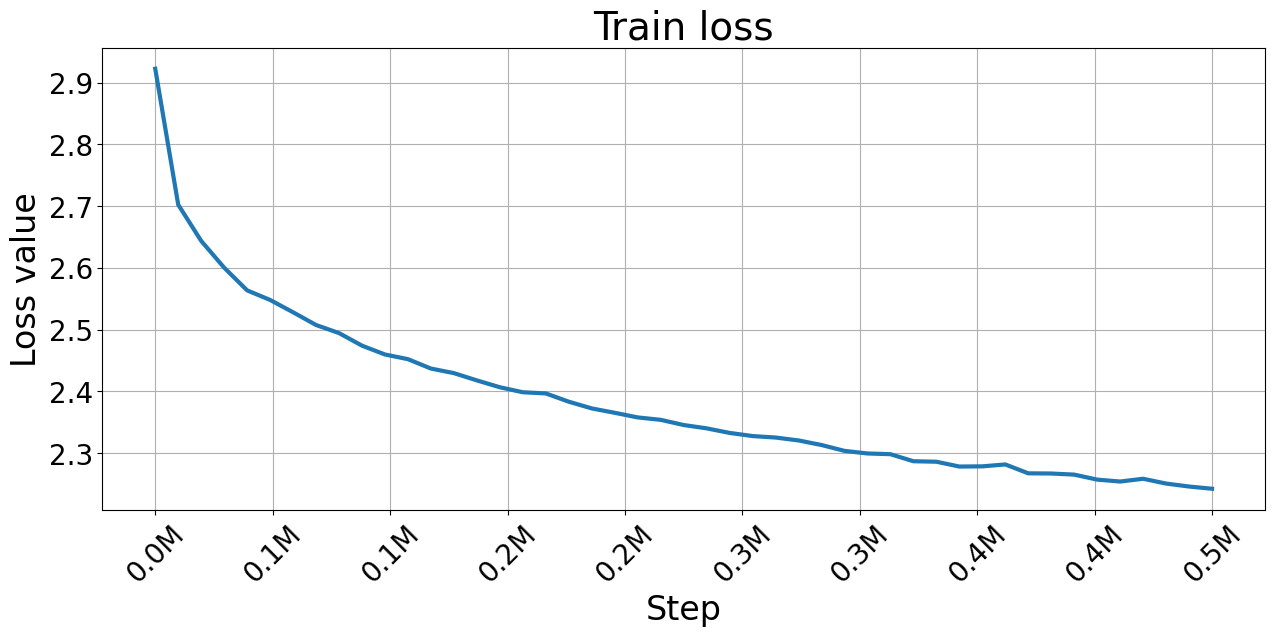
\includegraphics[scale=0.35]{figs/t5big_train_loss.png} \\
    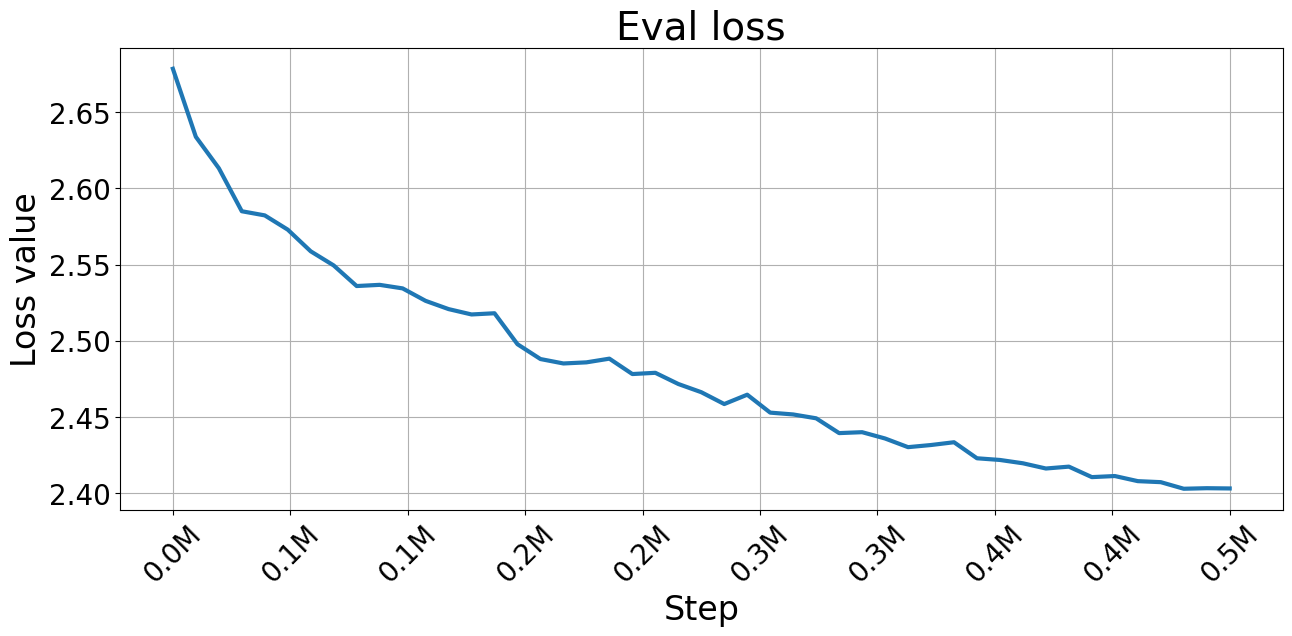
\includegraphics[scale=0.35]{figs/t5big_eval_loss.png}
    \caption{Loss history for CodeT5+ 770M.}
    ~\label{fig:big_model_loss}
\end{figure}

From Fig.~\ref{fig:big_model_loss}, it is easy to see that the training converges for the data splits of the training and evaluation. It should be noted that the model achieves better loss results across all splits. This means that the scaling transformer-based model in terms of parameters helps to achieve better results for the generation of commit messages. 

\begin{figure}[H]
    % \hspace*{-1.5cm}
    \centering
    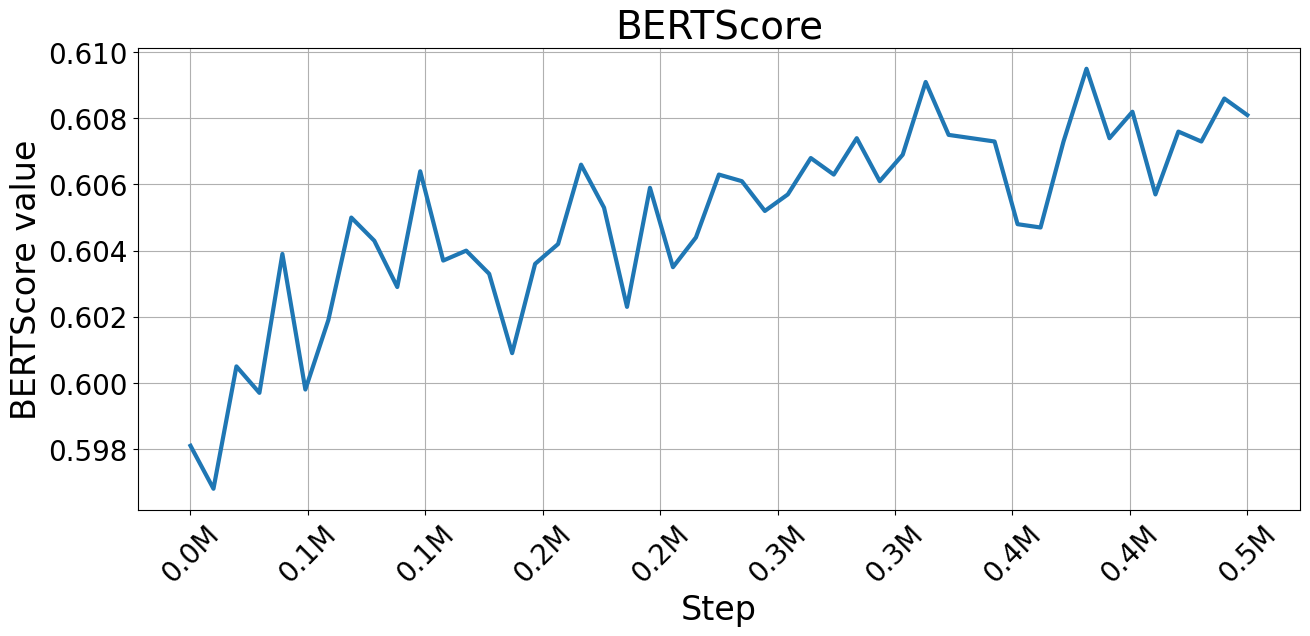
\includegraphics[scale=0.35]{figs/big_BERTScore.png} \\
    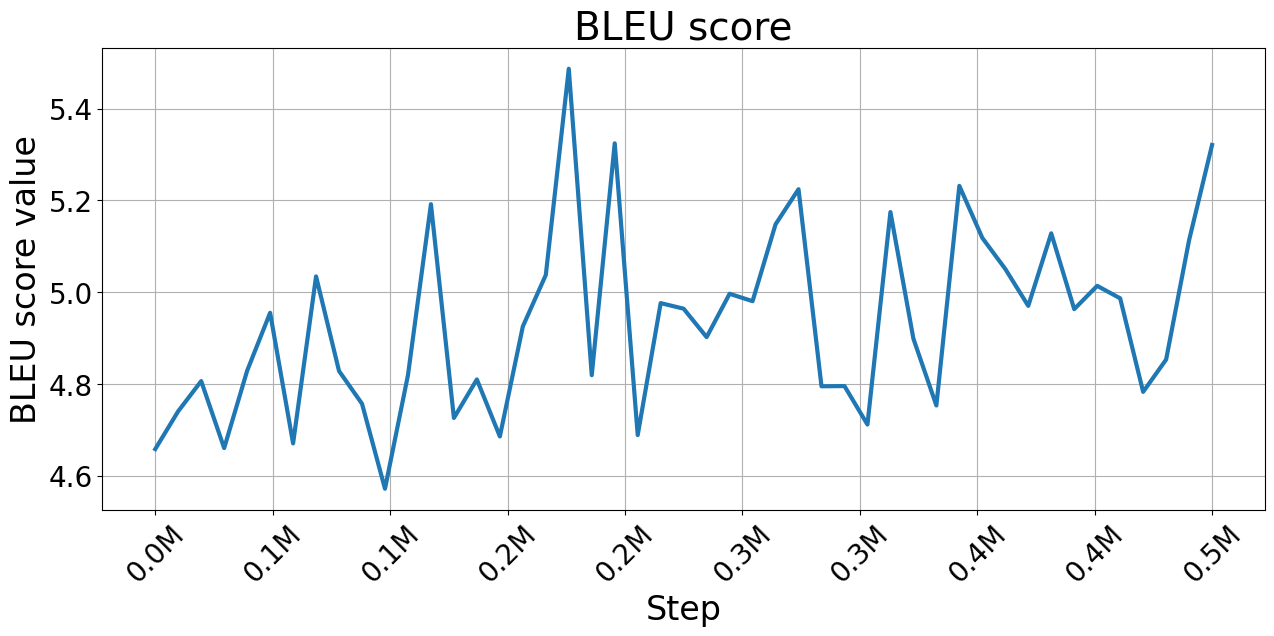
\includegraphics[scale=0.35]{figs/big_BLEU score.png} \\
    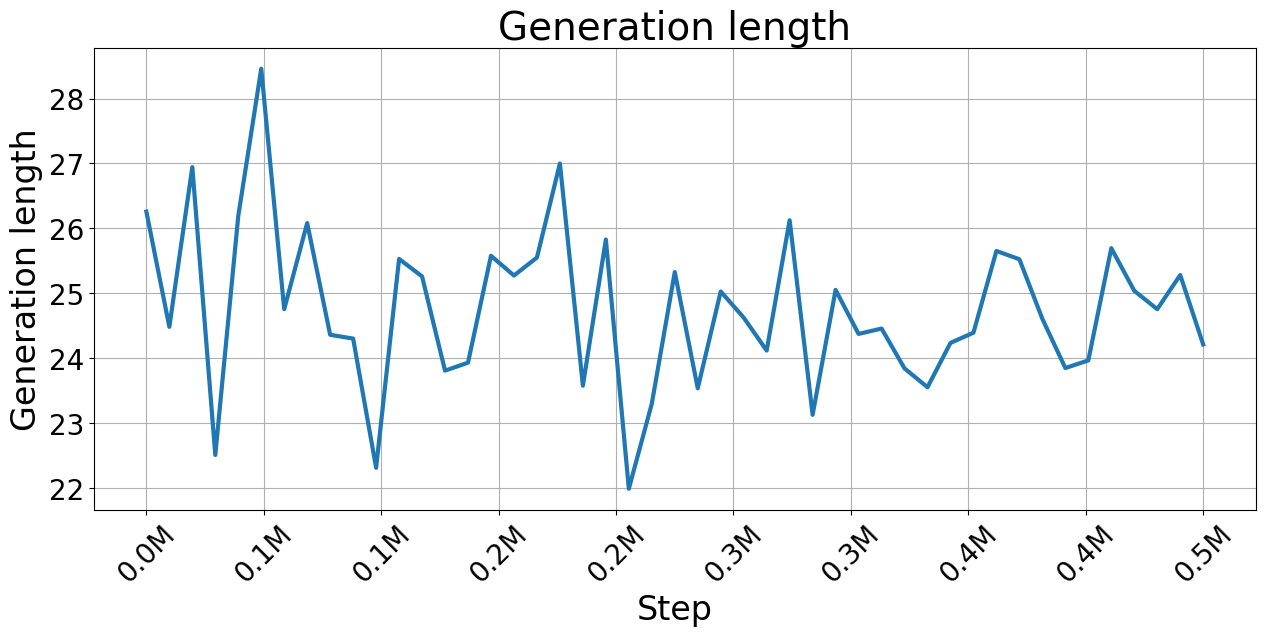
\includegraphics[scale=0.35]{figs/big_Generation length.png}
    \caption{Evaluation results for CodeT5+ 770M.}
    ~\label{fig:val_metrics_big}
\end{figure}
\newpage
Considering the evaluation results for the bigger model presented in Fig.~\ref{fig:val_metrics_big}, it also shows improvement of the generation quality during the fine-tuning. For the BERTScore computation in this experiment, I used a more powerful model for the embedding calculation. Therefore, the metric range is lower than for the base version. However, this metric improved during training and therefore the quality of the generated messages improved. BLEU score shows better results for this model and even has some tendency to grow, in contrast to the base CodeT5+ model. The ability of the model to generate more concise messages is also improved. It is visible from the average generation length plot. CodeT5+ with 770M parameters learned to generate messages with 24 tokens, compared to 31 for the base version.
In conclusion, I can say that the use of a deeper model with more stacked transformer blocks improved the performance of the target task. However, there is still a gap in the analysis of the model in terms of computational cost, GPU memory consumption, and inference time for the big model. In the evaluation chapter, I will analyze all the models from the efficiency perspective and make a judgment call on whether or not to use a scalled version of the model for the CMG task. 

\section{Training of CodeT5+ with retrieval}
\subsection{Architecture implementation details}
In this section, I will give details of the implementation of the experiment with the retrieved context. The motivation for the usage of the retrieval module and the design of the model architecture was described in~\ref{subsec:retrieval_arch_method}, so here I will focus on the practical part. The general pipeline of the model is presented in Fig.~\ref{fig:retrieval_pipeline}. In summary, the whole pipeline consists of the following steps: 1)Process the input batch of data, 2)Get the previous commit message from the same repository, 3)Using the embedding of code modifications, find the most similar commit and take its message, and 4)Using all the information construct the new batch and process it with base CodeT5+ like in the first experiment.
\begin{figure}[H]
    % \hspace*{-1.5cm}
    \centering
    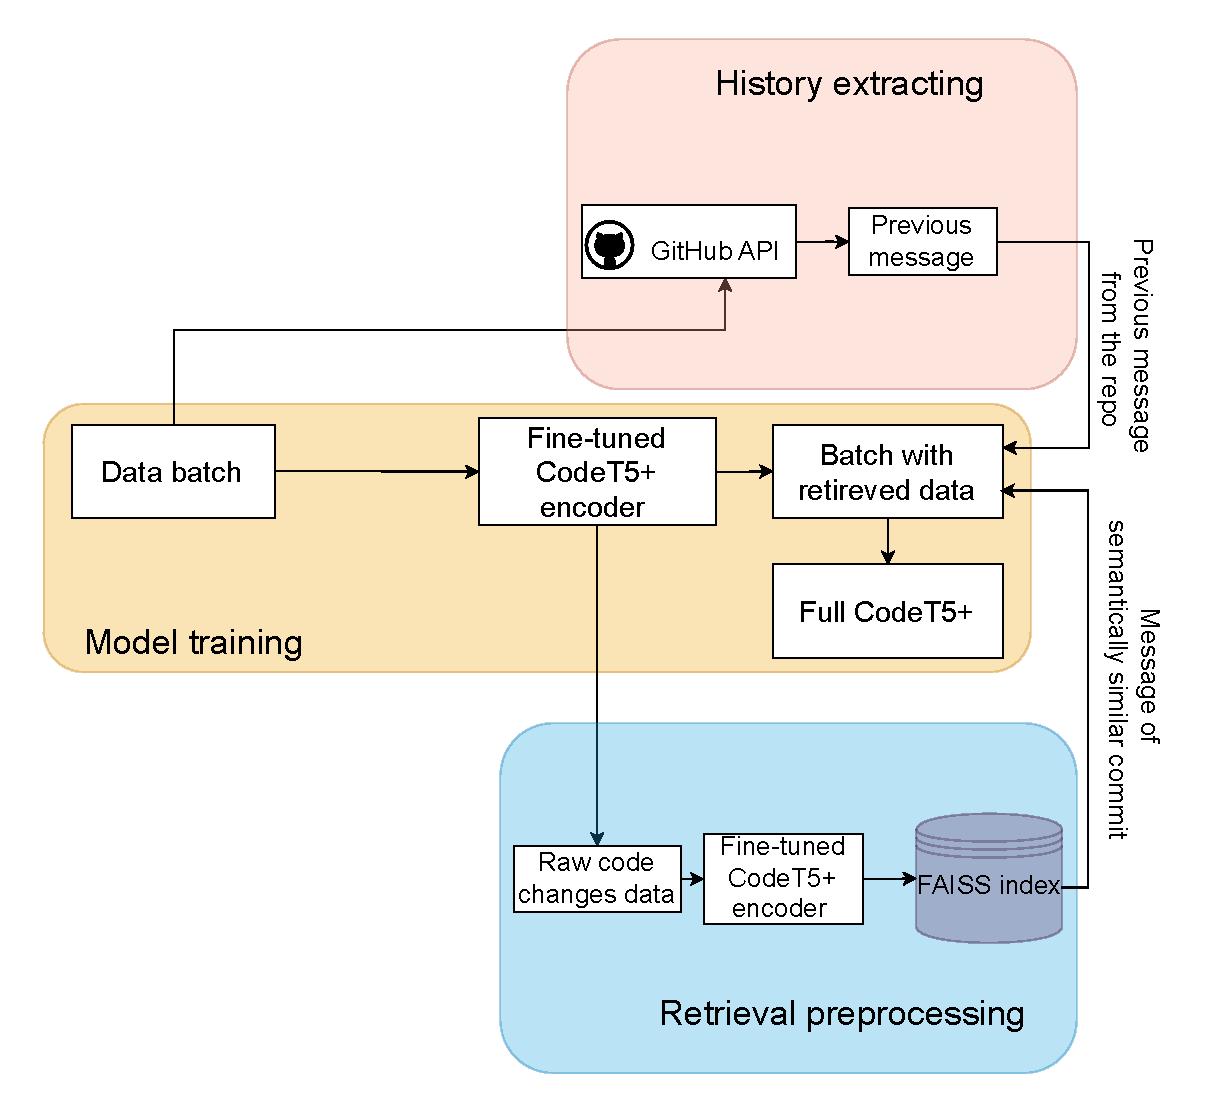
\includegraphics[scale=0.75]{figs/retrieval_arch.drawio.pdf}
    \caption{Architecture description for CodeT5+ with retrieval.}
    ~\label{fig:retrieval_pipeline}
\end{figure}
To retrieve previous messages from the same repository for a given commit, I utilized two different approaches for training and inference. During training and validation, I already had all the commits from the repository in the corresponding dataset split. Therefore, all I had to do was sort my dataset in order to map the samples with respect to time. During training, I precomputed all the necessary steps in advance and passed the previous message as an additional input field. On the other hand, during the inference time, I have live-time access only to the GitHub link to the commit. For this reason, I need to get the previous commit during the inference time. I used GitHub API to get the parent commit of the given.

To retrieve the message from the most similar code changes, I was required to have a precomputed database of embeddings from the training dataset. For this purpose, I processed the input split of the CommitChronicle with the encoder part of the pre-trained CodeT5+ from my first experiment. With a straightforward approach to finding the most similar commit at each forward pass, I need to calculate the cosine similarity between the input embedding and all the database embeddings.   This approach takes too much computation, so I need an approach to find the closest embedding to the given in a faster way. For this purpose, I used the FAIS~\cite{johnson2019billion} retrieval index, which can efficiently find the k closest points to the given in the high-dimensional data. Furthermore, this framework can make all computations on the GPU, thus making them parallelizable and faster. I have also experimented with another popular retrieval index - Annoy~\cite{annoy}, and found that FAIS is more precise and efficient.

Table~\ref{tab:retrieval_hyperparams} shows the hyperparameters for this specific retrieval architecture. The parameter \textbf{top\_k\_search} is responsible for the number of retrieved passages. According to the pipeline architecture, the model takes only one similar commit from the database. However, some passages can be considered irrelevant during the filtration phase. The retrieved commits must have been made after the given one. This filtration is crucial during model training, as it prevents overfitting by restricting the model from looking into the future and possible commits on the same code. One more filtration parameter is $\epsilon$ - cosine similarity threshold. This parameter is responsible for not including too similar commits, avoiding accidental retrieval of the target message. One more hyperparameter is the \textbf{max\_msg\_tokens}. As mentioned earlier, the transformer model has a limited context window size. Therefore, when I expand the input with previous and similar messages as the raw text, I need to control the length of the inserted data. I do not know the size of the retrieved context in advance. To prevent the context window from being overwhelmed by messages, I truncated the retrieved passages after a certain number of tokens.

\begin{table}[h]
    \centering
    \caption{Retrieval specific hyperparameters}\label{tab:retrieval_hyperparams}
    \renewcommand{\arraystretch}{1.5} % Adjusts the row height
    \begin{tabular}{| c | c |} % chktex 44
    \hline
    Hyperparameter & value \\ \hline  
    top\_k\_search & $20$ \\ \hline
    max\_msg\_tokens & $50$ \\ \hline
    $\epsilon$ & $0.1$ \\ \hline
    \end{tabular}
\end{table}

\subsection{Results of the training}
This section includes the results of CodeT5+ training with the retrieval module. Fig.~\ref{fig:retrieval_loss_hist} represents the loss history on the train and the validation data. From the plots, it is visible that the loss is decreasing during fine-tuning. It is important to note that even if the validation loss is in the same range as in the previous experiments, the loss for the train set is significantly lower than it was before. This behavior of the training loss may signal overfitting, meaning that the retrieved passage is close to the target message and the model trains to use it instead of looking into the code. However, validation loss is decreasing, so the model is generalized in the ability to generate commit messages.
\begin{figure}[H]
    % \hspace*{-1.5cm}
    \centering
    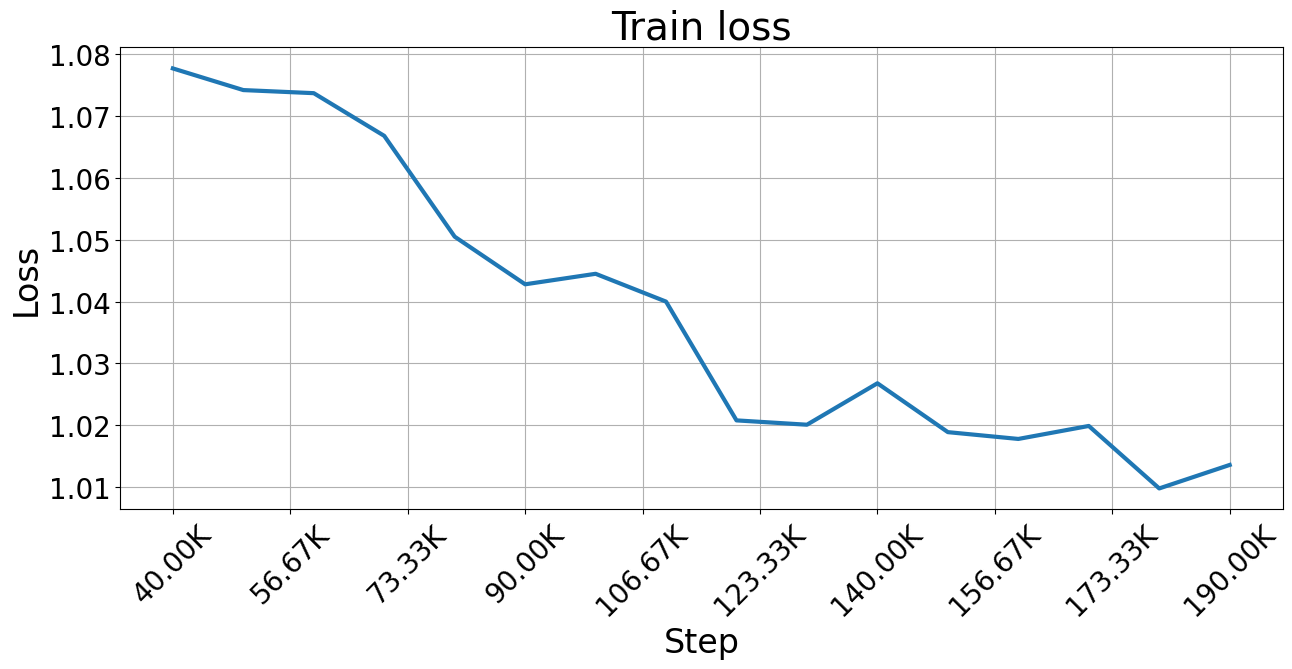
\includegraphics[scale=0.4]{figs/retrieval_Train loss.png}
    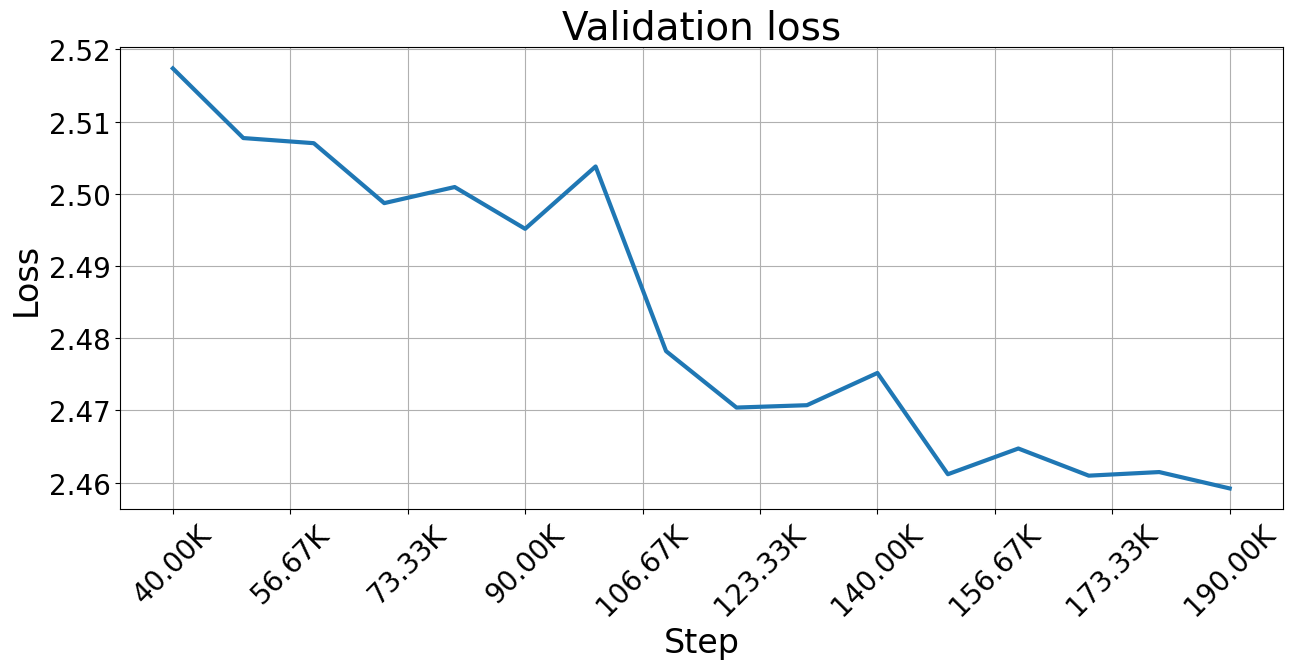
\includegraphics[scale=0.4]{figs/retrieval_Validation loss.png}
    \caption{Loss history for CodeT5+ with retrieval.}
    ~\label{fig:retrieval_loss_hist}
\end{figure}
Fig.~\ref{fig:retrieval_interim_metrics} represents the results of validation for CodeT5+ with the retrieval. BERTScore metric improved during training, but not significantly, from $0.6$ to $0.604$. BLEU score did not improve, even though it was the main goal to follow the style of the human-written message. However, the validation set is only a small subset of the original data. Thus, I need to have a full set evaluation to make sure that the experiment did not succeed. From the perspective of the generated sequence length, the model learned to construct shorter messages. Concluding this section I can say that the results from the small validation subset are unpersuasive, but to see the full picture and make a final decision about the experiment's importance I need to have a full evaluation.  
\begin{figure}[H]
    % \hspace*{-1.5cm}
    \centering
    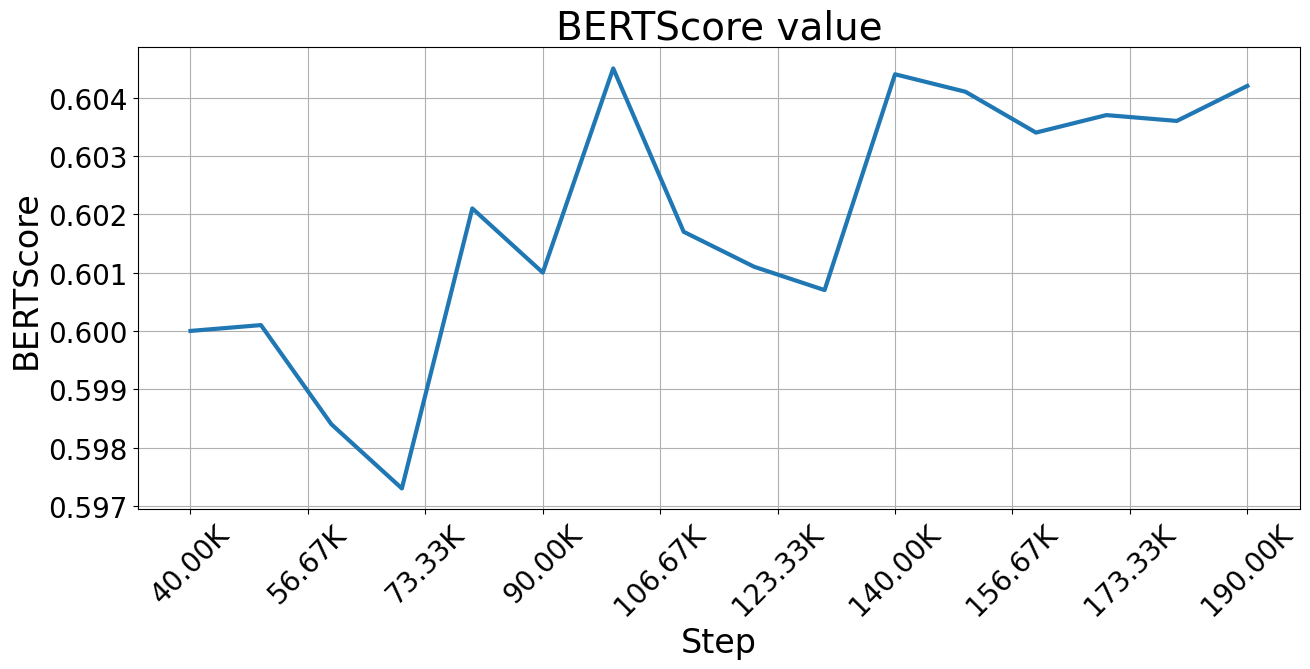
\includegraphics[scale=0.3]{figs/retrieval_BERTScore.png}
    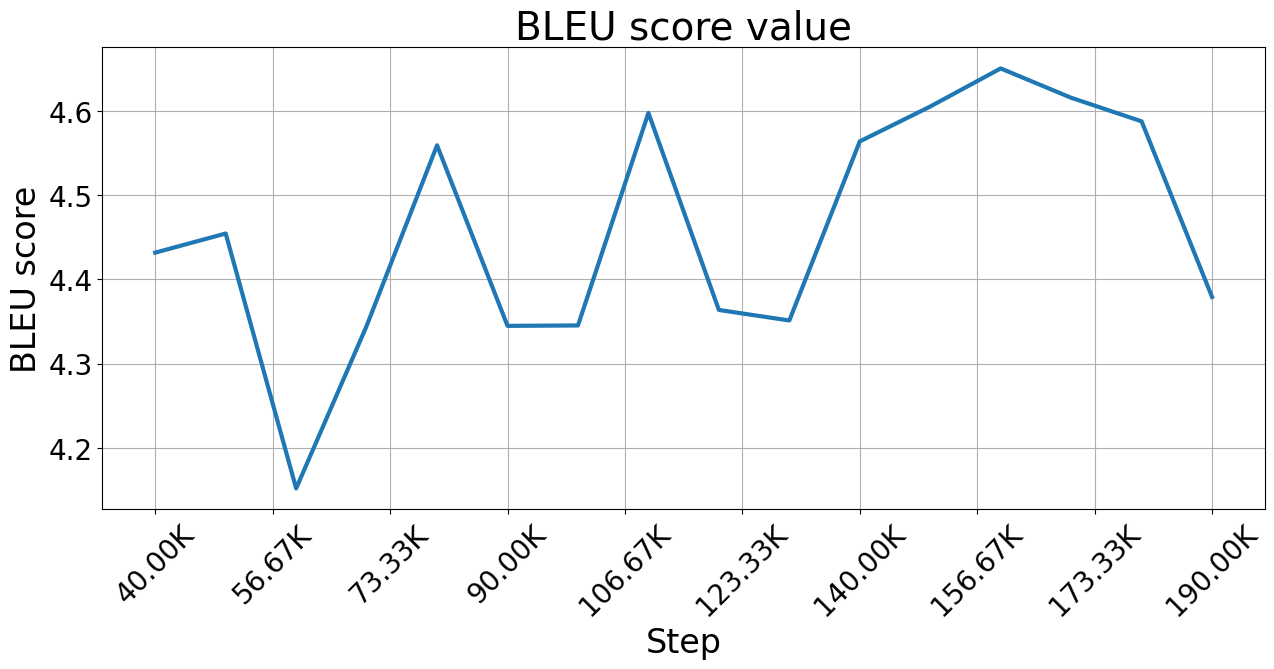
\includegraphics[scale=0.3]{figs/retrieval_BLEU score.png}
    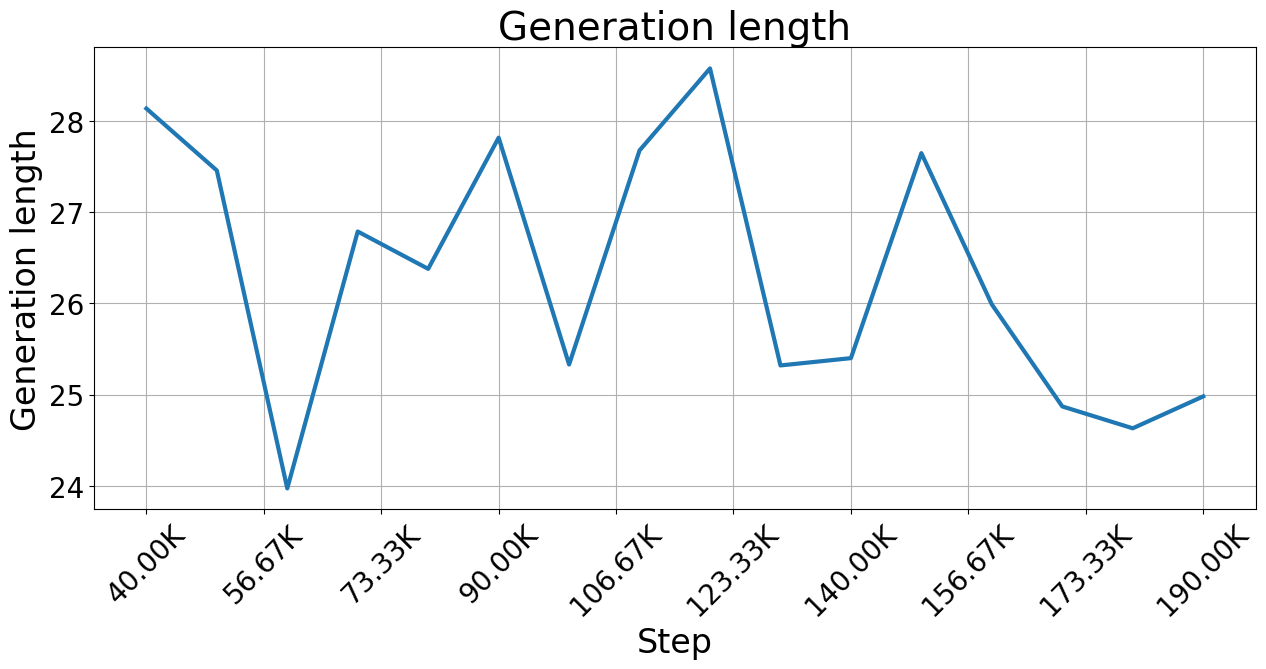
\includegraphics[scale=0.3]{figs/retrieval_Generation length.png}
    \caption{Loss history for CodeT5+ with retrieval.}
    ~\label{fig:retrieval_interim_metrics}
\end{figure}

\section{Training of CodeT5+ with file attention}

\subsection{Model architecture details}\label{subsec:fileattn_arch_details}

\begin{figure}[H]
    % \hspace*{-1.5cm}
    % \centering
    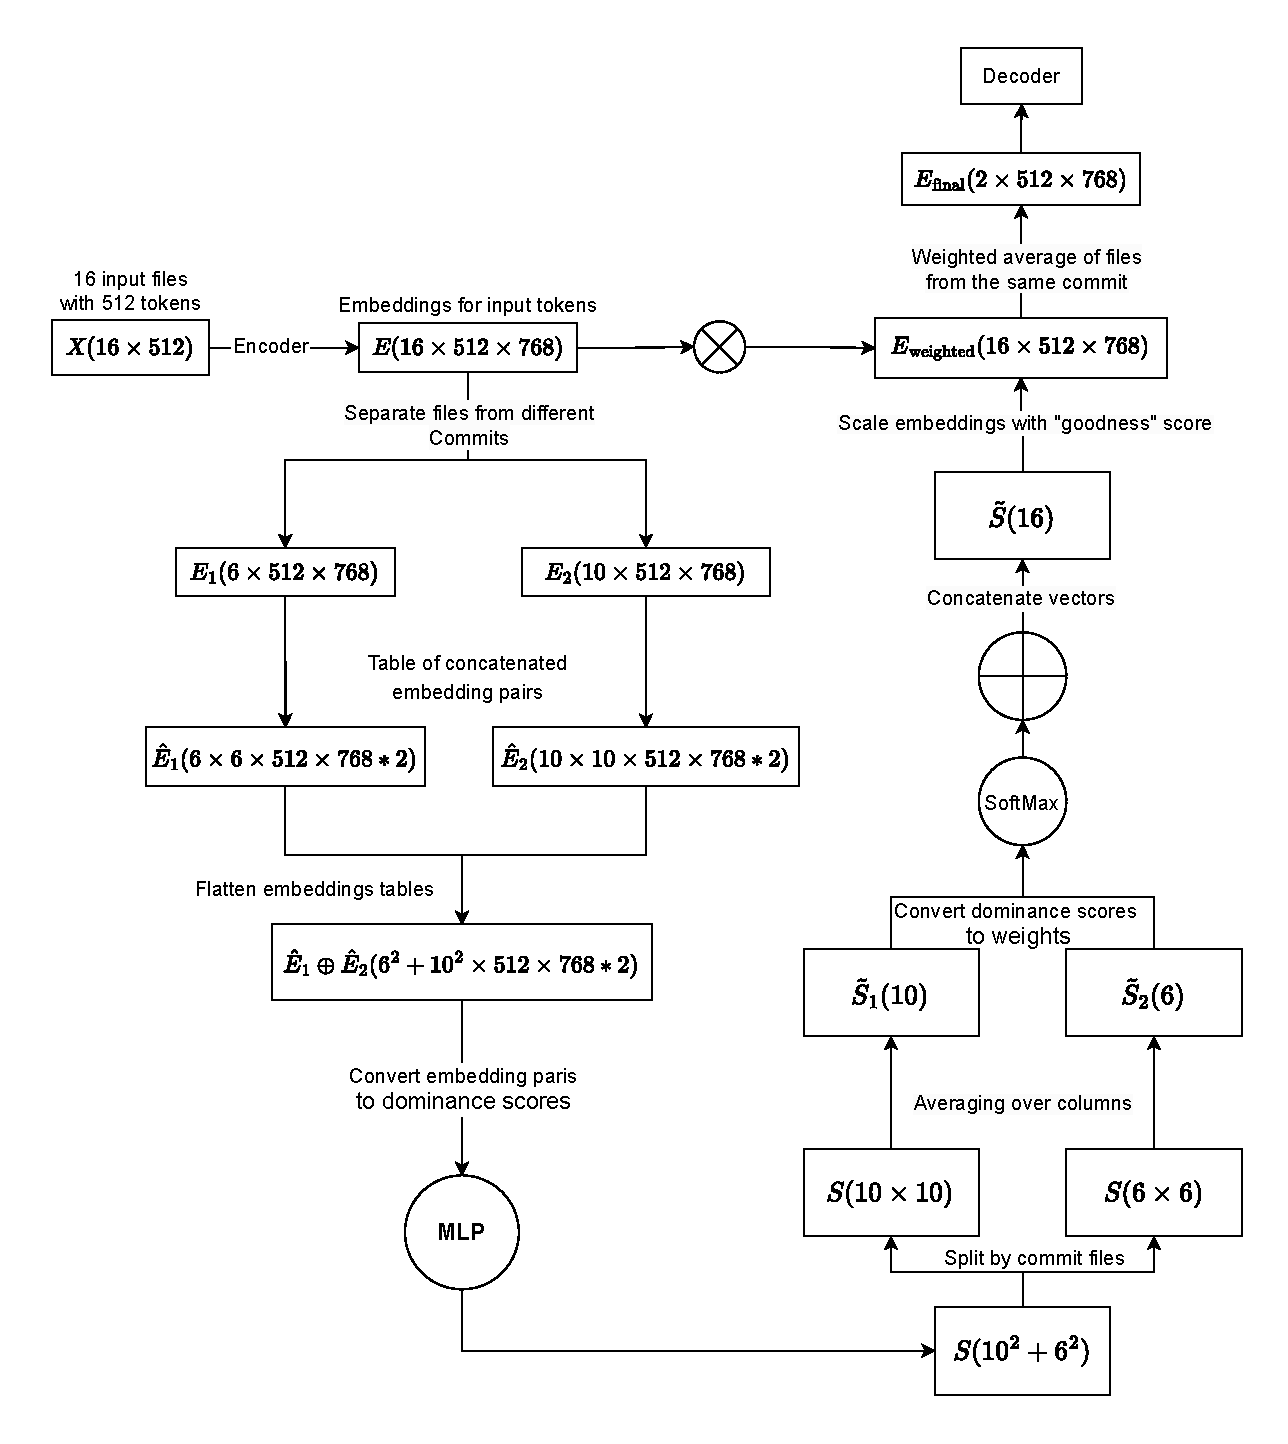
\includegraphics[scale=0.75]{figs/arch_v5.drawio.pdf}
    \caption{Architecture description for CodeT5+ with File attention.}
    ~\label{fig:file_attention_pipeline}
\end{figure}

\begin{figure}[H]   
    % \hspace*{-1.5cm}
    \centering
    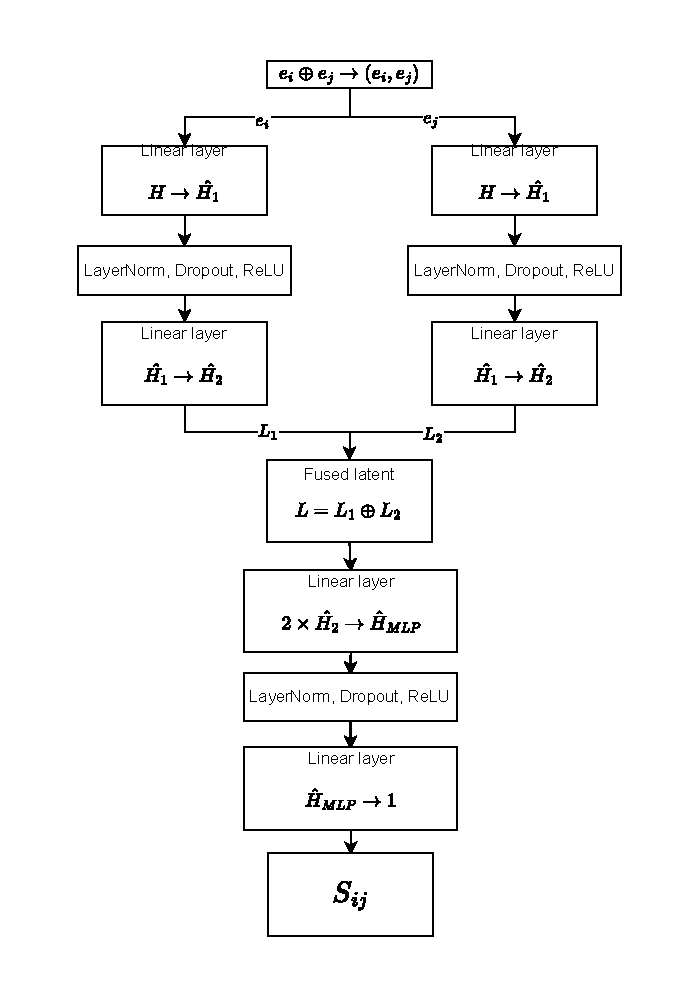
\includegraphics[scale=1]{figs/MLP_arch.pdf}
    \caption{Architecture of the MLP block.}
    ~\label{fig:file_attention_MLP_arch}
\end{figure}

This section includes the model implementation and training details for CodeT5+ with file attention. The model architecture follows the idea described in the methodology section~\ref{sec:file_attention_arch}. The overall pipeline of the model forward pass consists of the following steps:
\begin{enumerate}
    \item Taking the input in the format of the matrix of tokens of size $(n, m)$ where m is the context window of the CodeT5+ and n corresponds to the number files with the code changes in the batch. Each commit is separated by the files at the beginning. For example, the model takes a batch of $16$ files, where the first $6$ files correspond to the first commit and the remaining $10$ to the second. 
    \item Each file is passed through the encoder and produces embeddings matrix $E$ of the shape $(n, m, h)$, where $h$ is the hidden dimension of the model. For this experiment I used the fine-tuned version of the codeT5+ model, thus the encoder part is frozen and does not train. 
    \item The embedding matrix is separated by the commits. For each commit in the batch, I took the corresponding files and considered their embeddings separately. 
    \item For each embedding matrix, the model constructs the tensor of pairwise concatenated embeddings for each file from commit. It has a shape of $(n, n, m, h \times 2)$. It consists of all possible variants of embedding concatenations.
    \item Concatenated embeddings for all commits are flattened and then passed to the multi-layer perceptron \textbf{ (MLP)} block. Flattening is used to parallelize the computation of the \textbf{MLP}. The feedforward block of the neural network aims to determine the superiority score of code change file $i$ over file $j$ for each file pair. The architecture of the MLP block is presented in Fig.~\ref{fig:file_attention_MLP_arch}. Initially, the model splits back the concatenated embeddings for files $i$ and $j$ to consider them separately. Both embeddings are further mapped into the latent space using two linear layers with normalization activation and dropout between them. In the next step, latent vectors are fused and passed to the two linear layers resulting in one scalar - dominance score $S_{ij}$. This value represents how much file $i$ is "better" than file $j$.  
    \item In the previous step, the model produced vector $S$ of the shape $(n_1^2 + n_2^2)$, where $n_1$ and $n_2$ are numbers of files in the first and the second commit from the batch respectively. Each element in the $S$ represents the comparison of all possible pairs of files for every commit in the batch. In the next step, the model breaks this sequence to obtain a separate matrix with dominance scores for each commit. These matrices are then averaged by columns resulting with vector $\tilde{S}_i$ with size $n_i$ for each commit. For the given commit this vector represents how useful is the certain file with code changes within the scope of this commit. 
    \item The main purpose of this method is to have a trainable weighted sum of the embeddings over the files. To convert $\tilde{S}_i$ into weights it is passed through the Softmax function to have a distribution of usefulness among the files. 
    \item On the next step all the $\tilde{S}_i$ are fused into one vector $\tilde{S}$. This vector represents coefficients for the weighted average of the files embeddings for each commit. Applying weighted average to the initial embeddings matrix results with an embeddings matrix for the commits, which can be passed to the decoder in a regular way.   
\end{enumerate}
This procedure of averaging separate file embeddings instead of truncating the input increase the model performance in the case of long commits with multiple files. Moreover, all the operations performed between the encoder and decoder parts of the model are parallelized and does not affect the speed of the generation. Detailed analysis of the performance and time efficiency for all the model used in my work is presented in the evaluation chapter~\ref{chap:eval}

\subsection{Training setup details}
The training setup for this model is different from other experiments. The input batch for the file attention model consists of a fixed number of code files. Therefore, the number of commits in a single batch may vary. The dataset entry contains a single commit that may include up to $16$ changed files. For training, I decided to have the data in batches with $16$ files. For batch construction, I iterated over the dataset and included the commit in the batch if the number of files did not exceed the fixed maximum number. Thus, before the start of the training, I had pre-computed batches.
Commit data may vary among the samples. They may contain different programming languages or project semantics. The backward pass through the MLP block has a united gradient for the whole batch. This property of the unified gradient may break the correct training of the weights for the importance of the files. To handle this possible drawback, I did an additional experiment with a single commit in the batch. This setup reduces the parallelism of the training, but it can improve the model's ability to determine the relevance of files within a commit.

\subsection{Training results}
This section presents the results of the training for both setups described above. As in the previous experiments, it includes the loss convergence in training and validation sets.
During the training phase, the implementation of inference mechanisms for this architecture was not ready. Consequently, this section will not encompass a discussion of the metric evaluations for the training checkpoints. A comprehensive analysis of the quality of the generated commits will be included in the subsequent evaluation chapter.

\begin{figure}[H]   
    % \hspace*{-1.5cm}
    \centering
    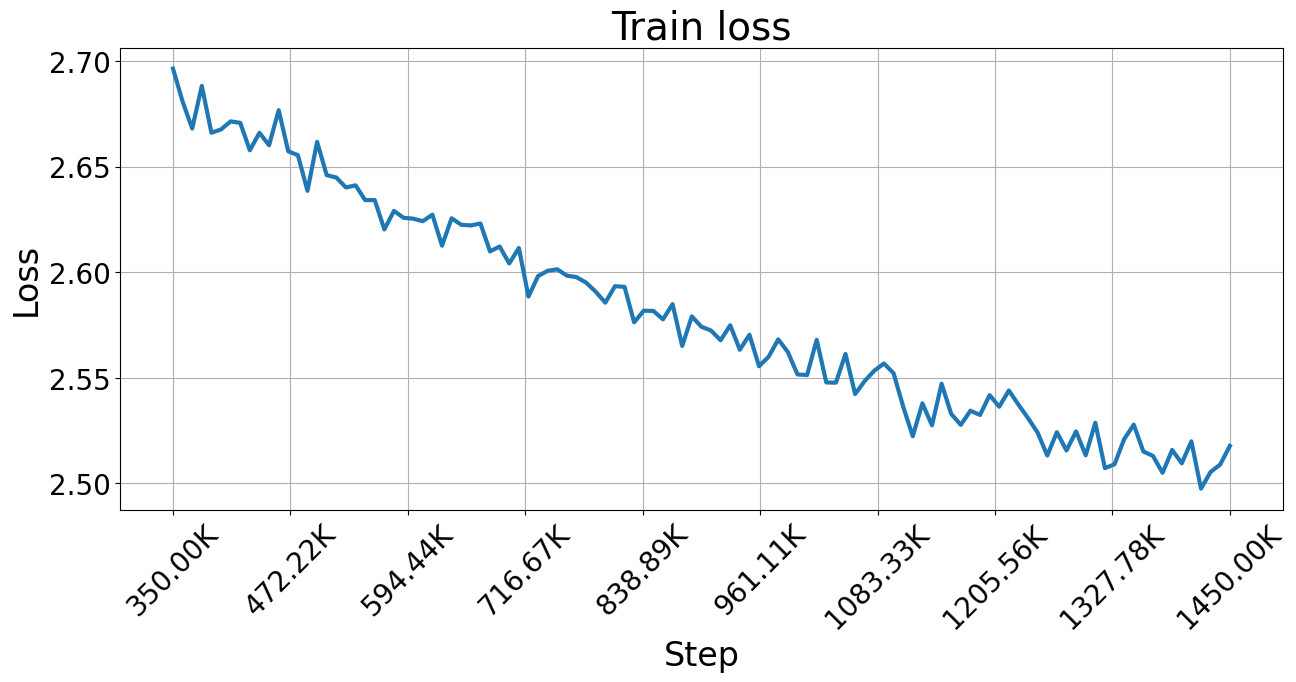
\includegraphics[scale=0.4]{figs/file_attn_train_loss.png}
    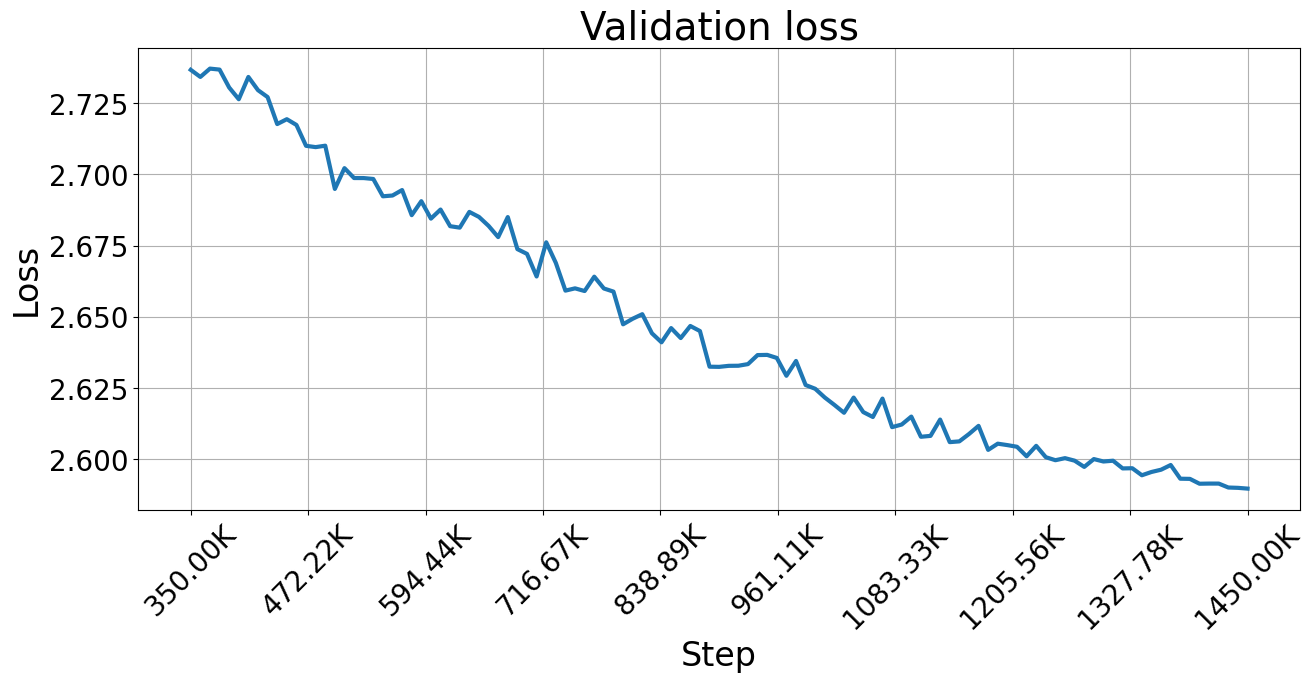
\includegraphics[scale=0.4]{figs/file_attn_val_loss.png}
    \caption{Loss history for CodeT5+ with file attention.}
    ~\label{fig:loss_hist_file_attn}
\end{figure}

Fig.~\ref{fig:loss_hist_file_attn} represents the trajectory of loss convergence for the CodeT5+ model incorporating the file attention mechanism.
The plots clearly illustrate that the loss trajectories for both datasets are monotonically decreasing, indicating that the fine-tuning process has been successful and the model has effectively acquired the capability to generate commit messages. However, considering only the intermediate loss values is not sufficient to draw a conclusion about the model performance.  

\begin{figure}[H]   
    % \hspace*{-1.5cm}
    \centering
    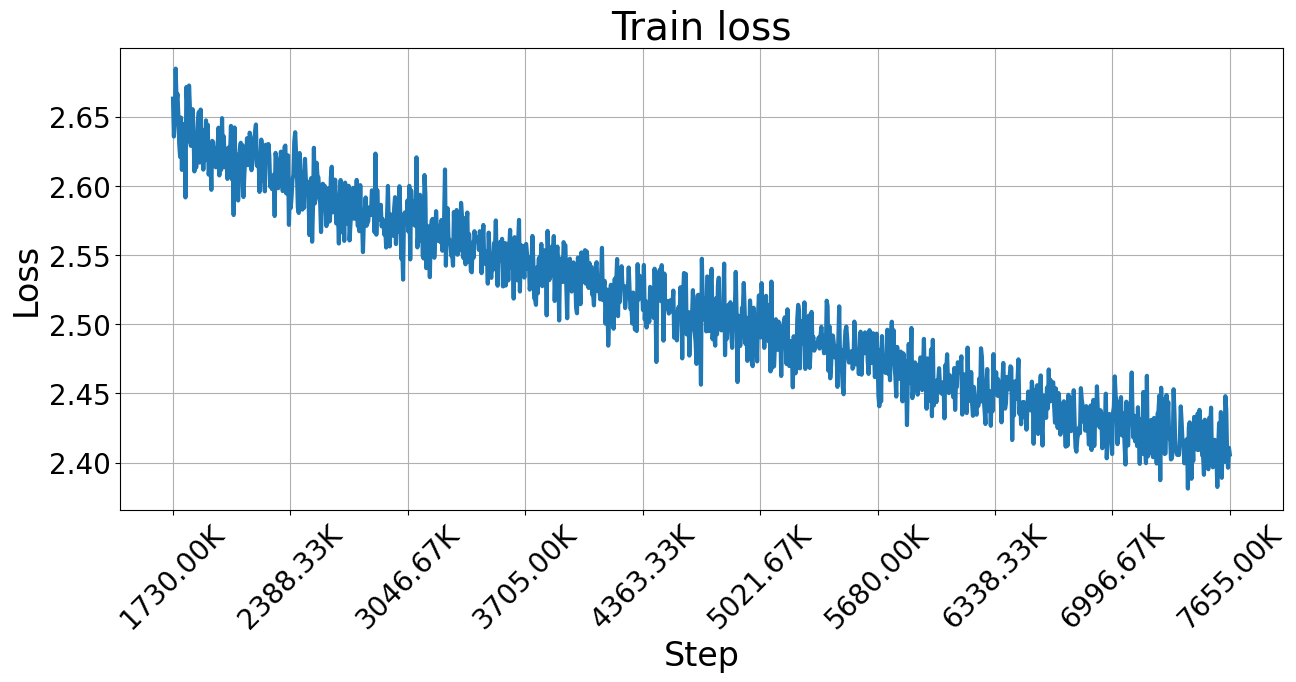
\includegraphics[scale=0.4]{figs/file_attn_train_loss_single.png}
    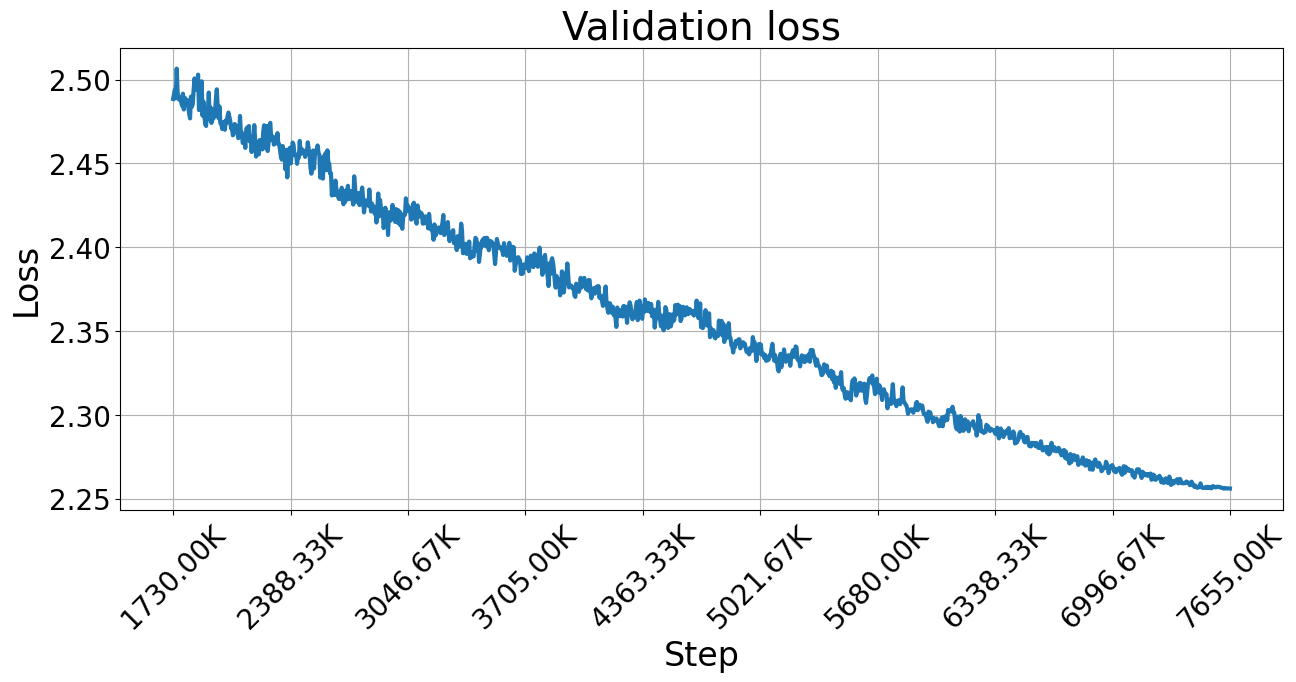
\includegraphics[scale=0.4]{figs/file_attn_val_loss_single.png}
    \caption{Loss history for CodeT5+ with file attention.}
    ~\label{fig:loss_hist_file_attn_single}
\end{figure}

The convergence of the loss function for the secondary configuration, with a single commit within the batch, is depicted in Fig.~\ref{fig:loss_hist_file_attn_single}. Plots shows that this setup shows better convergence for the validation loss. In contrast to the initial configuration, which has multiple commits per batch and ends up with a final validation loss approximately equal to 2.60, the second setup employing a single commit shows a better loss, achieving approximately 2.25. Furthermore, the loss metrics for the training data are also improved in the second configuration. However, the possible reason for this may be the greater number of backward steps. As visible from the plots, in the setup with a batched input, 1.45M steps were made during fine tuning. At the same time, using a single commit as an input, the model takes 7.655M steps to fine-tune on the whole dataset. This significant difference in the training samples also affected the fine-tuning time. While the first version took approximately 5 days to train, the second one required almost 11 days for the full fine-tuning process.
In summarizing this comparative analysis, it is evident that relying only on the values of the loss function is insufficient to make a judgment regarding the performance of the model in different setups. A comprehensive evaluation of training methodologies requires the analysis of metrics derived from the test data to ensure a fair comparison. 